%杨舒云的实验报告编辑界面,使用了Huanyu Shi,2019级的模板,杨舒云在此拜谢ORZ!

%!TEX program = xelatex
\documentclass[dvipsnames, svgnames,a4paper,11pt]{article}
% ----------------------------------------------------- 
%	加边框的命令
%	参考:https://tex.stackexchange.com/questions/531559/how-to-add-the-page-border-for-first-two-pages-in-latex
\usepackage{tikz}
\usetikzlibrary{calc}
\usepackage{eso-pic}
\AddToShipoutPictureBG{%
\begin{tikzpicture}[overlay,remember picture]
\draw[line width=0.6pt] % 边框粗细
    ($ (current page.north west) + (0.6cm,-0.6cm) $)
    rectangle
    ($ (current page.south east) + (-0.6cm,0.6cm) $); % 边框位置
\end{tikzpicture}}


\usepackage{xcolor}
\definecolor{c1}{HTML}{086173} % 目录颜色 原版为2752C9 紫灰色535AAA 蓝紫色0B0DB7 深蓝色070F94 湖绿色219394 松石灰绿086173
\definecolor{c2}{HTML}{E20129} % 引用颜色 原版\definecolor{c2}{RGB}{190,20,83} 橙色F24729

\usepackage{ctex}
\usepackage[top=28mm,bottom=28mm,left=15mm,right=15mm]{geometry}
\usepackage{hyperref} 
\hypersetup{
	colorlinks,
	linktoc = section, % 超链接位置,选项有section, page, all
	linkcolor = c1, % linkcolor 目录颜色
	citecolor = c1  % citecolor 引用颜色
}
\usepackage{amsmath,enumerate,multirow,float}
\usepackage{tabularx}
\usepackage{tabu}
\usepackage{subfig}
\usepackage{fancyhdr}
\usepackage{graphicx}
\usepackage{wrapfig}  
\usepackage{physics}
\usepackage{appendix}
\usepackage{amsfonts}

%
\usepackage{tcolorbox}
\tcbuselibrary{skins,breakable}
\newtcolorbox{tbox}[2][]{
    colframe=black!70!,
    breakable,
    enhanced,
	boxrule =0.5pt,
    title = {#2},
    fonttitle = \large\kaishu\bfseries,
	drop fuzzy shadow,
    #1
}
\newtcolorbox[auto counter,number within=section]{question}[1][]{
  top=2pt,bottom=2pt,arc=1mm,
  boxrule=0.5pt,
%   frame hidden,
  breakable,
  enhanced, %跨页后不会显示下边框
  coltitle=c1!80!gray,
  colframe=c1,
  colback=c1!3!white,
  drop fuzzy shadow,
  title={思考题~\thetcbcounter:\quad},
  fonttitle=\bfseries,
  attach title to upper,
  #1
}

% ---------------------------------------------------------------------
%	利用cleveref改变引用格式,\cref是引用命令
\usepackage{cleveref}
\crefformat{figure}{#2{\textcolor{c2}{Figure #1}}#3} % 图片的引用格式
\crefformat{equation}{#2{(\textcolor{c2}{#1})}#3} % 公式的引用格式
\crefformat{table}{#2{\textcolor{c2}{Table #1}}#3} % 表格的引用格式


% ---------------------------------------------------------------------
%	页眉页脚设置
\fancypagestyle{plain}{\pagestyle{fancy}}
\pagestyle{fancy}
\lhead{\kaishu 中山大学物理与天文学院电子技术实验\uppercase\expandafter{\romannumeral1}} % 左边页眉,学院 + 课程
\rhead{\kaishu 实验报告By杨舒云\&戴鹏辉} % 右边页眉,实验报告标题
\cfoot{\thepage} % 页脚,中间添加页码


% ---------------------------------------------------------------------
%	对目录、章节标题的设置
\renewcommand{\contentsname}{\centerline{\huge 目录}}
\usepackage{titlesec}
\usepackage{titletoc}
% \titleformat{章节}[形状]{格式}{标题序号}{序号与标题间距}{标题前命令}[标题后命令]
\titleformat{\section}{\centering\LARGE\songti}{}{1em}{}

% ---------------------------------------------------------------------
%   listing代码环境设置
\usepackage{listings}
\lstloadlanguages{python}
\lstdefinestyle{pythonstyle}{
backgroundcolor=\color{gray!5},
language=python,
frameround=tftt,
frame=shadowbox, 
keepspaces=true,
breaklines,
columns=spaceflexible,                   
basicstyle=\ttfamily\small, % 基本文本设置,字体为teletype,大小为scriptsize
keywordstyle=[1]\color{c1}\bfseries, 
keywordstyle=[2]\color{Red!70!black},   
stringstyle=\color{Purple},       
showstringspaces=false,
commentstyle=\ttfamily\scriptsize\color{green!40!black},%注释文本设置,字体为sf,大小为smaller
tabsize=2,
morekeywords={as},
morekeywords=[2]{np, plt, sp},
numbers=left, % 代码行数
numberstyle=\it\tiny\color{gray}, % 代码行数的数字字体设置
stepnumber=1,
rulesepcolor=\color{gray!30!white}
}




% ---------------------------------------------------------------------
%	其他设置
\def\degree{${}^{\circ}$} % 角度
\graphicspath{{./images/}} % 插入图片的相对路径
\allowdisplaybreaks[4]  %允许公式跨页 
\usepackage{lipsum}
\usepackage{adjustbox}
%\usepackage{mathrsfs} % 字体
\captionsetup[figure]{name=Figure} % 图片形式
\captionsetup[table]{name=Table} % 表格形式
\usepackage{tabularray} % 添加关于绘制表格的包

\begin{document}
	
	
	
	% 实验报告封面	
	
	% 顶栏
	\begin{table}
		\renewcommand\arraystretch{1.7}
		\begin{tabularx}{\textwidth}{
				|X|X|X|X
				|X|X|X|X|}
			\hline
			\multicolumn{2}{|c|}{预习报告}&\multicolumn{2}{|c|}{实验记录}&\multicolumn{2}{|c|}{分析讨论}&\multicolumn{2}{|c|}{总成绩}\\
			\hline
			\LARGE25 & & \LARGE25 & & \LARGE30 & & \LARGE80 & \\
			\hline
		\end{tabularx}
	\end{table}
	% ---
	
	% 信息栏
	\begin{table}
		\renewcommand\arraystretch{1.7}
		\begin{tabularx}{\textwidth}{|X|X|X|X|}
			\hline
			年级、专业: & 2022级 物理学 &组号: & E2\\
			\hline
			姓名: & 戴鹏辉、杨舒云  & 学号: & 22344016、22344020\\
			\hline
			实验时间: & 2024/3/27 & 教师签名: & \\
			\hline
		\end{tabularx}
	\end{table}
	% ---
	
	% 大标题
	\begin{center}
		\LARGE ET1-5 \quad 一阶电路暂态过程的研究
	\end{center}
	% ---
	
	% 注意事项
	
	% 基本
	\textbf{【实验报告注意事项】}
	\begin{enumerate}
		\item 实验报告由三部分组成:
		\begin{enumerate}
			\item 预习报告:课前认真研读实验讲义,弄清实验原理;实验所需的仪器设备、用具及其使用、完成课前预习思考题;了解实验需要测量的物理量,并根据要求提前准备实验记录表格(可以参考实验报告模板,可以打印)。\textcolor{red}{\textbf{(20分)}}
			\item 实验记录:认真、客观记录实验条件、实验过程中的现象以及数据。实验记录请用珠笔或者钢笔书写并签名(\textcolor{red}{\textbf{用铅笔记录的被认为无效}})。\textcolor{red}{\textbf{保持原始记录,包括写错删除部分,如因误记需要修改记录,必须按规范修改。}}(不得输入电脑打印,但可扫描手记后打印扫描件);离开前请实验教师检查记录并签名。\textcolor{red}{\textbf{(30分)}}
			\item 数据处理及分析讨论:处理实验原始数据(学习仪器使用类型的实验除外),对数据的可靠性和合理性进行分析;按规范呈现数据和结果(图、表),包括数据、图表按顺序编号及其引用;分析物理现象(含回答实验思考题,写出问题思考过程,必要时按规范引用数据);最后得出结论。\textcolor{red}{\textbf{(30分)}}
		\end{enumerate}
		\textbf{实验报告就是将预习报告、实验记录、和数据处理与分析合起来,加上本页封面。\textcolor{red}{(80分)}}
		\item 每次完成实验后的一周内交\textbf{实验报告}(特殊情况不能超过两周)。
		\item \textbf{其它注意事项}:
		\begin{enumerate}
			\item 请认真查看并理解实验讲义第一章内容;
			\item 注意实验器材的合理使用;
			\item 使用结束使用各种仪器之后需要将其放回原位。
		\end{enumerate}
	\end{enumerate}
	
	% 安全
	\textbf{【实验安全注意事项】}	
	\begin{enumerate}
		\item 电路左端为输入端,加方波信号,右端为输出端,接示波器,不要弄错。
		\item 用示波器观察波形,一定要将输入信号选择开关置于“AC”位置,随被测信号幅值不同,改变幅值开关的位置,使波形清晰可测。
		
	\end{enumerate}
	
	% ---
	
	% 特别鸣谢
	\textbf{【特别鸣谢及模板说明】}	
	
	感谢2019级学长石寰宇为本实验报告提供\LaTeX 模板。\textcolor{red}{\textbf{由于原实验报告模板缺少实验编号,为方便在电脑上整理,故添加自命名编号}}
	% ---
	
	
	
	% 目录
	\clearpage
	\tableofcontents
	\clearpage
	% ---
	
	
	
	% 预习报告	
	
	% 小标题
	\setcounter{section}{0}
	\section{ET1-5 一阶电路暂态过程的研究 \quad\heiti 预习报告}
	% ---
	
	% 实验目的
	\subsection{实验目的}
	\begin{enumerate}
		\item 研究一阶电路的零输入响应,零状态响应及全响应的基本规律和特点。
		\item 学习一阶电路时间常数τ的测量方法。
		\item 熟悉微分和积分电路结构,加深对构成微分和积分电路必要条件的理解。
		\item 进一步熟悉应用示波器进行电参数测量的方法。
		
	\end{enumerate}
	% ---
	
	% 仪器用具
	\subsection{仪器用具}
	\begin{table}[htbp]
		\centering
		\renewcommand\arraystretch{1.6}
		% \setlength{\tabcolsep}{10mm}
		\begin{tabular}{p{0.05\textwidth}|p{0.20\textwidth}|p{0.05\textwidth}|p{0.5\textwidth}}
			\hline
			编号& 仪器用具名称 & 数量 &  主要参数(型号,测量范围,测量精度等) \\
			\hline
			1& 电路原理箱或板 & 1 & 一阶电路动态过程的研究 \\
			\hline
			2& 示波器 & 1 &  \\
			\hline
			3& 2号实验导线 & n & 二端2号镀金插头  \\
			\hline

		\end{tabular}
	\end{table}
	% ---
	
	% 原理概述
	\subsection{原理概述}
	\begin{enumerate}
		\item \textbf{动态电路及响应}:含有L、C元件的电路称为动态电路,其描述方程为微分方程。线性电路的响应可分为零状态响应、零输入响应及全响应,分别由初始条件和激励引起。

		\item \textbf{一阶电路}:电路中只含有一个电感或电容元件时称为一阶电路。一阶电路的零输入响应按指数规律衰减,零状态响应按指数规律递增或递减,速率由电路参数确定的时间常数$\tau$决定。
		
		\item \textbf{过渡过程}:动态电路的过渡过程是短暂的单次变化过程,难以直接观察。常用方法是用方波仪记录过程,根据电路时间常数$\tau$的大小采用不同的实验方法。
		
		\item \textbf{微分电路和积分电路}:微分电路和积分电路是脉冲数字电路中常见的波形变换电路。当电路时间常数$\tau$远小于或远大于方波脉冲宽度$T_p$时,微分电路可将方波变换成尖脉冲,积分电路可将方波变换成三角波。
	\end{enumerate}
	% ---
	
	% 实验前思考题
	\subsection{实验预习题}
	
	% 思考题1
	\begin{question}
		微分电路如图\ref*{fig:graph1}所示,R=5.1KΩ,$C_2$=0.1μF,试问对方波脉宽有什么要求?
	\end{question}



		在微分电路中,方波脉宽的要求与电路的时间常数$\tau$有关。时间常数是由电阻$R$和电容$C$的值决定的,计算公式为$ \tau = R \times C$。对于此电路,R = 5.1KΩ 和 $C_1$​ = 0.1μF,时间常数 $\tau$ 可以计算如下:
		\[
			\tau=R\times C_1​=5.1\times10^3\Omega×0.1×10^{−6}F=5.1×10^{−4}s
		\]
		
		在微分电路中,为了使电路正常工作,方波的脉宽$Tp$应远大于电路的时间常数,通常至少是时间常数的20倍以上。这样,电路才能对输入信号进行有效的微分。如果方波脉宽太短,电容将无法在每个脉冲之间充分放电,导致输出信号失真。
		则对于此电路,方波脉宽的要求大致为:
		\[
			Tp\gg20\tau=20×5.1×10^{−4}s=10.2ms
		\]
		
		这意味着方波脉宽应远大于10.2ms才能确保电路正常工作。

		\begin{figure}[htbp]
			\centering
			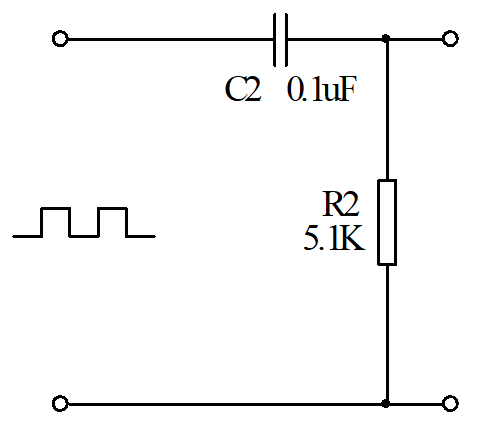
\includegraphics[width=0.4\textwidth]{graph1.png}
			\caption{RC微分电路}
			\label{fig:graph1}
		\end{figure}



	% % 思考题2
	% \begin{question}
		
	% \end{question}
	
	% % 思考题3
	% \begin{question}
		
	% \end{question}
	
	% ---
	
	
	
	% 实验记录	
	\clearpage
	
	% 顶栏
	\begin{table}
		\renewcommand\arraystretch{1.7}
		\centering
		\begin{tabularx}{\textwidth}{|X|X|X|X|}
			\hline
			专业: & 物理学 & 年级: & 2022级 \\
			\hline
			姓名: & 戴鹏辉、杨舒云 & 学号: & 22344016、22344020\\
			\hline
			室温: & 25\degree C & 实验地点: & A522 \\
			\hline
			学生签名:& 见\textbf{附件}部分 & 评分: &\\
			\hline
			实验时间:& 2024/3/27 & 教师签名:&\\
			\hline
		\end{tabularx}
	\end{table}
	% ---
	
	% 小标题
	\section{ET1-5 一阶电路暂态过程的研究  \quad\heiti 实验记录}
	% ---
	
	% 实验过程记录
	\subsection{实验内容、步骤与结果}
	
	%
	\subsubsection{操作步骤记录}
	\begin{enumerate}
		\item 一阶电路的研究
		\begin{enumerate}
			\item 输入输出特性
			
			RC一阶电路是由一个电阻(R)和一个电容(C)串联组成的电路,其输入输出特性取决于输入信号的类型。如果输入是方波信号,那么输入输出特性会有一些特定的行为。
			
			\begin{enumerate}
				\item \textbf{输入信号:} 方波信号是一个周期性的信号,其波形是由两个离散电平构成的,一个高电平(通常表示逻辑1)和一个低电平(通常表示逻辑0)。方波信号的频率、占空比等参数可以根据具体的应用而变化。
				
				\item \textbf{输出特性:} 当方波信号输入到RC一阶电路中时,电路会有以下响应:
				\begin{enumerate}
					\item \textbf{充电阶段(Rising Edge):} 当方波信号从低电平变为高电平时,电容开始充电。在这个阶段,电容上的电压会逐渐增加,直到达到与输入电压相同的水平。充电的速度取决于电容和电阻的数值,以及输入信号的上升时间。
					
					\item \textbf{放电阶段(Falling Edge):} 当方波信号从高电平变为低电平时,电容开始放电。在这个阶段,电容上的电压会逐渐减小,直到达到与输入电压相同的水平。放电的速度同样取决于电容和电阻的数值,以及输入信号的下降时间。
				\end{enumerate}
				
				\item \textbf{输出波形:} 在RC一阶电路中,输出波形会随着输入方波信号的变化而变化。具体来说,输出波形会是一串由指数函数衰减的脉冲。在充电阶段,输出波形的上升边缘会经历一个指数增长的过程;而在放电阶段,输出波形的下降边缘会经历一个指数衰减的过程。
				
				\item \textbf{时间常数:} RC电路的特性还受到一个称为时间常数(τ)的影响,时间常数定义为RC的乘积,即 \( \tau = R \cdot C \)。时间常数决定了电容充电或放电的速度。当输入信号的变化时间远大于时间常数时,电容将有足够的时间来充电或放电,输出波形将可以完全跟随输入信号。反之,当输入信号的变化时间远小于时间常数时,电容将无法跟随输入信号的变化,输出波形可能会失真。
			\end{enumerate}
			
			RL一阶电路是由一个电阻(R)和一个电感(L)串联组成的电路,其输入输出特性也会受到输入信号类型的影响。如果输入是方波信号,那么输入输出特性会有一些特定的行为。
			
			\begin{enumerate}
				\item \textbf{输入信号:} 方波信号是一个周期性的信号,其波形由两个离散电平构成,一个高电平(通常表示逻辑1)和一个低电平(通常表示逻辑0)。方波信号的频率、占空比等参数可以根据具体的应用而变化。
				
				\item \textbf{输出特性:} 当方波信号输入到RL一阶电路中时,电路会有以下响应:
				\begin{enumerate}
					\item \textbf{上升边缘(Rising Edge):} 当方波信号从低电平变为高电平时,电感中的电流开始增加。在这个阶段,电感产生的感应电压会与输入电压叠加,导致输出电压上升。上升边缘的速度取决于电感和电阻的数值,以及输入信号的上升时间。
					
					\item \textbf{下降边缘(Falling Edge):} 当方波信号从高电平变为低电平时,电感中的电流开始减小。在这个阶段,电感产生的感应电压会与输入电压叠加,导致输出电压下降。下降边缘的速度同样取决于电感和电阻的数值,以及输入信号的下降时间。
				\end{enumerate}
				
				\item \textbf{输出波形:} 在RL一阶电路中,输出波形会随着输入方波信号的变化而变化。具体来说,输出波形会是一串由指数函数衰减的脉冲。在上升边缘阶段,输出波形的上升边缘会经历一个指数增长的过程;而在下降边缘阶段,输出波形的下降边缘会经历一个指数衰减的过程。
				
				\item \textbf{时间常数:} RL电路的特性还受到一个称为时间常数(τ)的影响,时间常数定义为RL的比值,即 \( \tau = \frac{L}{R} \)。时间常数决定了电感电流变化的速度。当输入信号的变化时间远大于时间常数时,电感将有足够的时间来响应输入信号的变化,输出波形将可以完全跟随输入信号。反之,当输入信号的变化时间远小于时间常数时,电感将无法跟随输入信号的变化,输出波形可能会失真。
			\end{enumerate}
			
			\item 测量时间常数
			
			\textbf{测量RC电路的时间常数:}
			
			\begin{enumerate}
				\item \textbf{准备工作:} 首先需要准备一个已知电阻值的电阻器(R)和一个已知电容值的电容器(C),以及一个可调频率的方波信号发生器、示波器、连接线等实验器材。
				
				\item \textbf{搭建电路:} 将电阻器和电容器串联连接,构成RC电路。连接方波信号发生器的输出端到电路的输入端,连接示波器的探头分别到电路的输入端和输出端。
				
				\item \textbf{调节方波信号频率:} 通过方波信号发生器调节方波信号的频率,使其适合实验需求,一般选择一个相对较低的频率。
				
				\item \textbf{观察示波器波形:} 调节示波器,观察输入信号和输出信号的波形。
				
				\item \textbf{测量时间常数:} 在示波器上测量输出波形上升或下降到原始值的时间(\textbf{37\%方波电压,利用示波器上AX和BX读数}),这个时间就是RC电路的时间常数($\tau$)。
				
				\item \textbf{记录数据:} 记录测得的时间常数值。
				
				\item \textbf{重复实验:} 为了提高测量准确度,可以多次重复以上步骤,取多次测量结果的平均值。
			\end{enumerate}
			
			\textbf{测量RL电路的时间常数:}
			
			\begin{enumerate}
				\item \textbf{准备工作:} 同样需要准备一个已知电阻值的电阻器(R)和一个已知电感值的电感线圈(L),以及一个可调频率的方波信号发生器、示波器、连接线等实验器材。
				
				\item \textbf{搭建电路:} 将电阻器和电感线圈串联连接,构成RL电路。连接方波信号发生器的输出端到电路的输入端,连接示波器的探头分别到电路的输入端和输出端。
				
				\item \textbf{调节方波信号频率:} 通过方波信号发生器调节方波信号的频率,使其适合实验需求,一般选择一个相对较低的频率。
				
				\item \textbf{观察示波器波形:} 调节示波器,观察输入信号和输出信号的波形。
				
				\item \textbf{测量时间常数:} 在示波器上测量输出波形上升或下降到原始值的时间(\textbf{37\%方波电压,利用示波器上AX和BX读数}),这个时间就是RL电路的时间常数($\tau$)。
				
				\item \textbf{记录数据:} 记录测得的时间常数值。
				
				\item \textbf{重复实验:} 为了提高测量准确度,可以多次重复以上步骤,取多次测量结果的平均值。
			\end{enumerate}
		\end{enumerate}
		
		\item 微分电路和积分电路的研究
		\begin{enumerate}
			\item RC微分电路:RC微分电路如\cref{fig:graph2}所示,调节方波仪输出频率,使方波脉冲宽度满足微分电路的必要条件,将R2、R4分别接入,观察微分电路输出有何不同。
			
			% \begin{figure}[htbp]
			% 	\centering
			% 	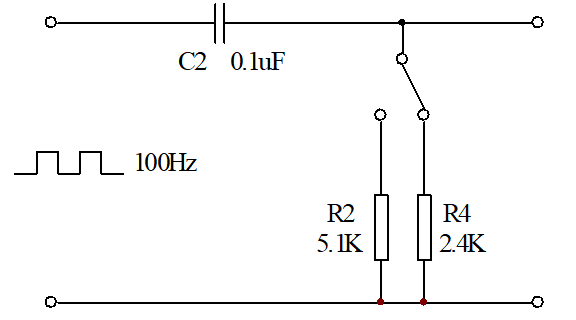
\includegraphics[width=0.4\textwidth]{graph2.png}
			% 	\caption{RC微分电路}
			% 	\label{fig:graph2}
			% \end{figure}
			
			\item RL微分电路:RL微分电路如\cref{fig:graph3}所示,调节方波仪输出频率,使方波脉冲宽度满足微分电路的必要条件,将R1、R3分别接入,观察微分电路输出有何不同。
			
			\begin{figure}[htbp]
				\centering
				\subfloat[RC微分电路]
				{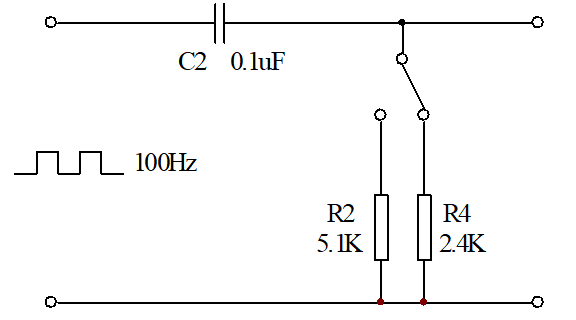
\includegraphics[width=0.35\textwidth]{graph2.png}\label{fig:graph2}}
				\quad
				\subfloat[$\tau=0.51ms$]
				{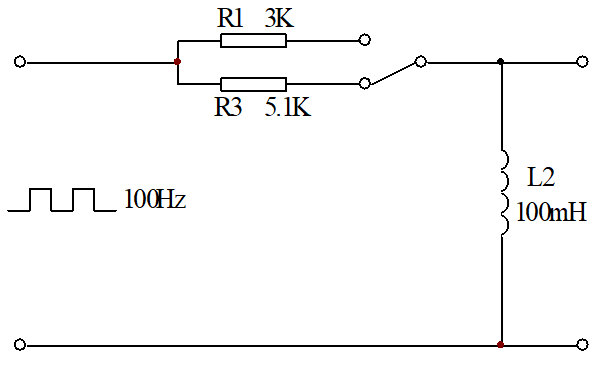
\includegraphics[width=0.35\textwidth]{graph3.png}\label{fig:graph3}}
				\quad
				\caption{RL微分电路}
				\label{fig:graph2-1}
			\end{figure}


			% \begin{figure}[htbp]
			% 	\centering
			% 	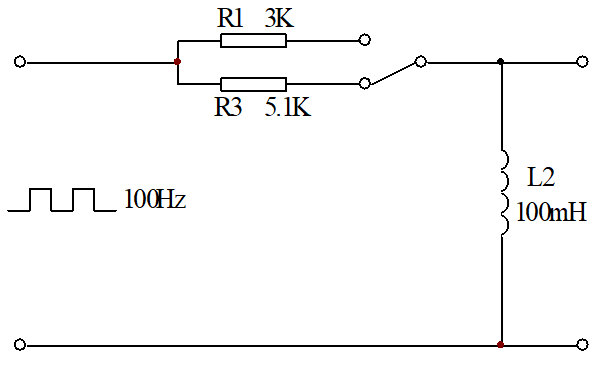
\includegraphics[width=0.4\textwidth]{graph3.png}
			% 	\caption{RL微分电路}
			% 	\label{fig:graph3}
			% \end{figure}
			
			\item RC积分电路:RC积分电路如\cref{fig:graph4}所示,在方波脉冲宽度满足积分电路必要条件下,将R1、R3分别接入,观察积分电路输出有何不同。
			
			% \begin{figure}[htbp]
			% 	\centering
			% 	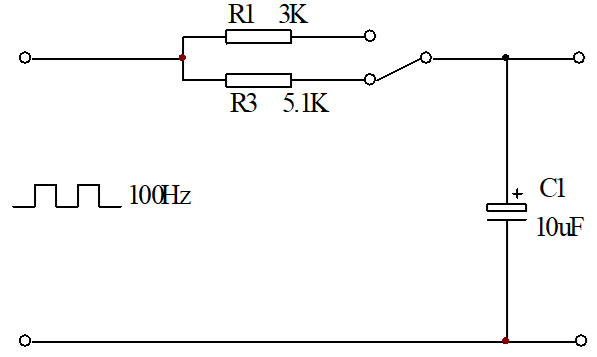
\includegraphics[width=0.4\textwidth]{graph4.png}
			% 	\caption{RC积分电路}
			% 	\label{fig:graph4}
			% \end{figure}
			
			\item RL积分电路:RL积分电路如\cref{fig:graph5}所示,在方波脉冲宽度满足积分电路必要条件下,将R2、R4分别接入,观察积分电路输出有何不同。
			
			\begin{figure}[htbp]
				\centering
				\subfloat[RC积分电路]
				{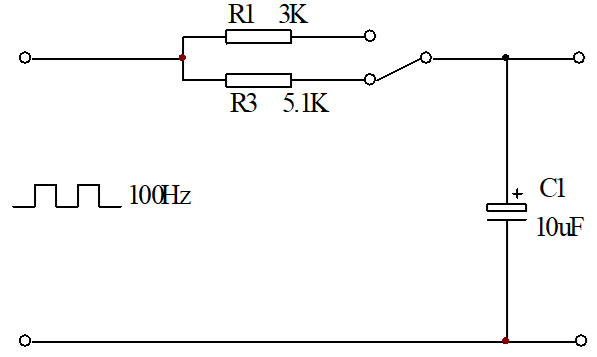
\includegraphics[width=0.35\textwidth]{graph4.png}\label{fig:graph4}}
				\quad
				\subfloat[$\tau=0.51ms$]
				{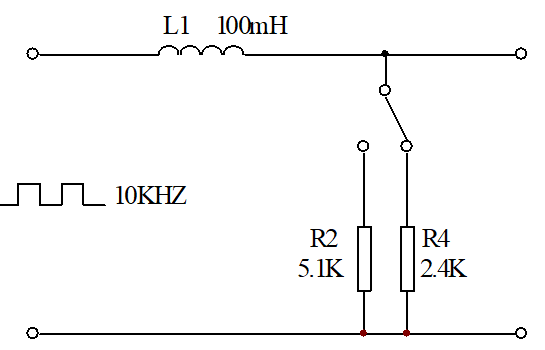
\includegraphics[width=0.35\textwidth]{graph5.png}\label{fig:graph5}}
				\quad
				\caption{RL积分电路}
				\label{fig:graph2-1}
			\end{figure}


			% \begin{figure}[htbp]
			% 	\centering
			% 	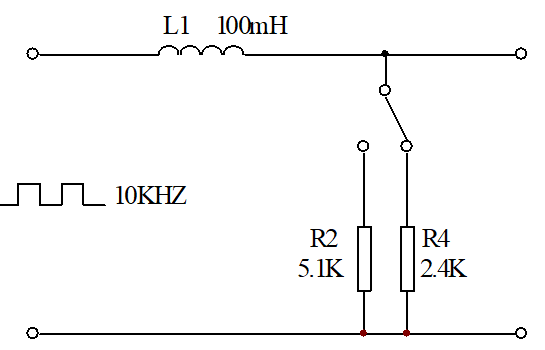
\includegraphics[width=0.4\textwidth]{graph5.png}
			% 	\caption{RL积分电路}
			% 	\label{fig:graph5}
			% \end{figure}
			
		\end{enumerate}
	\end{enumerate}	
	
	%
	\subsubsection{实验结果展示}
	\begin{enumerate}
		\item 输出波形展示
		
		RC微分电路,$C=0.1\mu F$,当$R=2.4k\Omega$时,输出波形如\cref{fig:graph2-11}所示;当$R=5.1k\Omega$时,输出波形如\cref{fig:graph2-12}所示。

		\begin{figure}[htbp]
			\centering
			\subfloat[$\tau=0.24ms$]
			{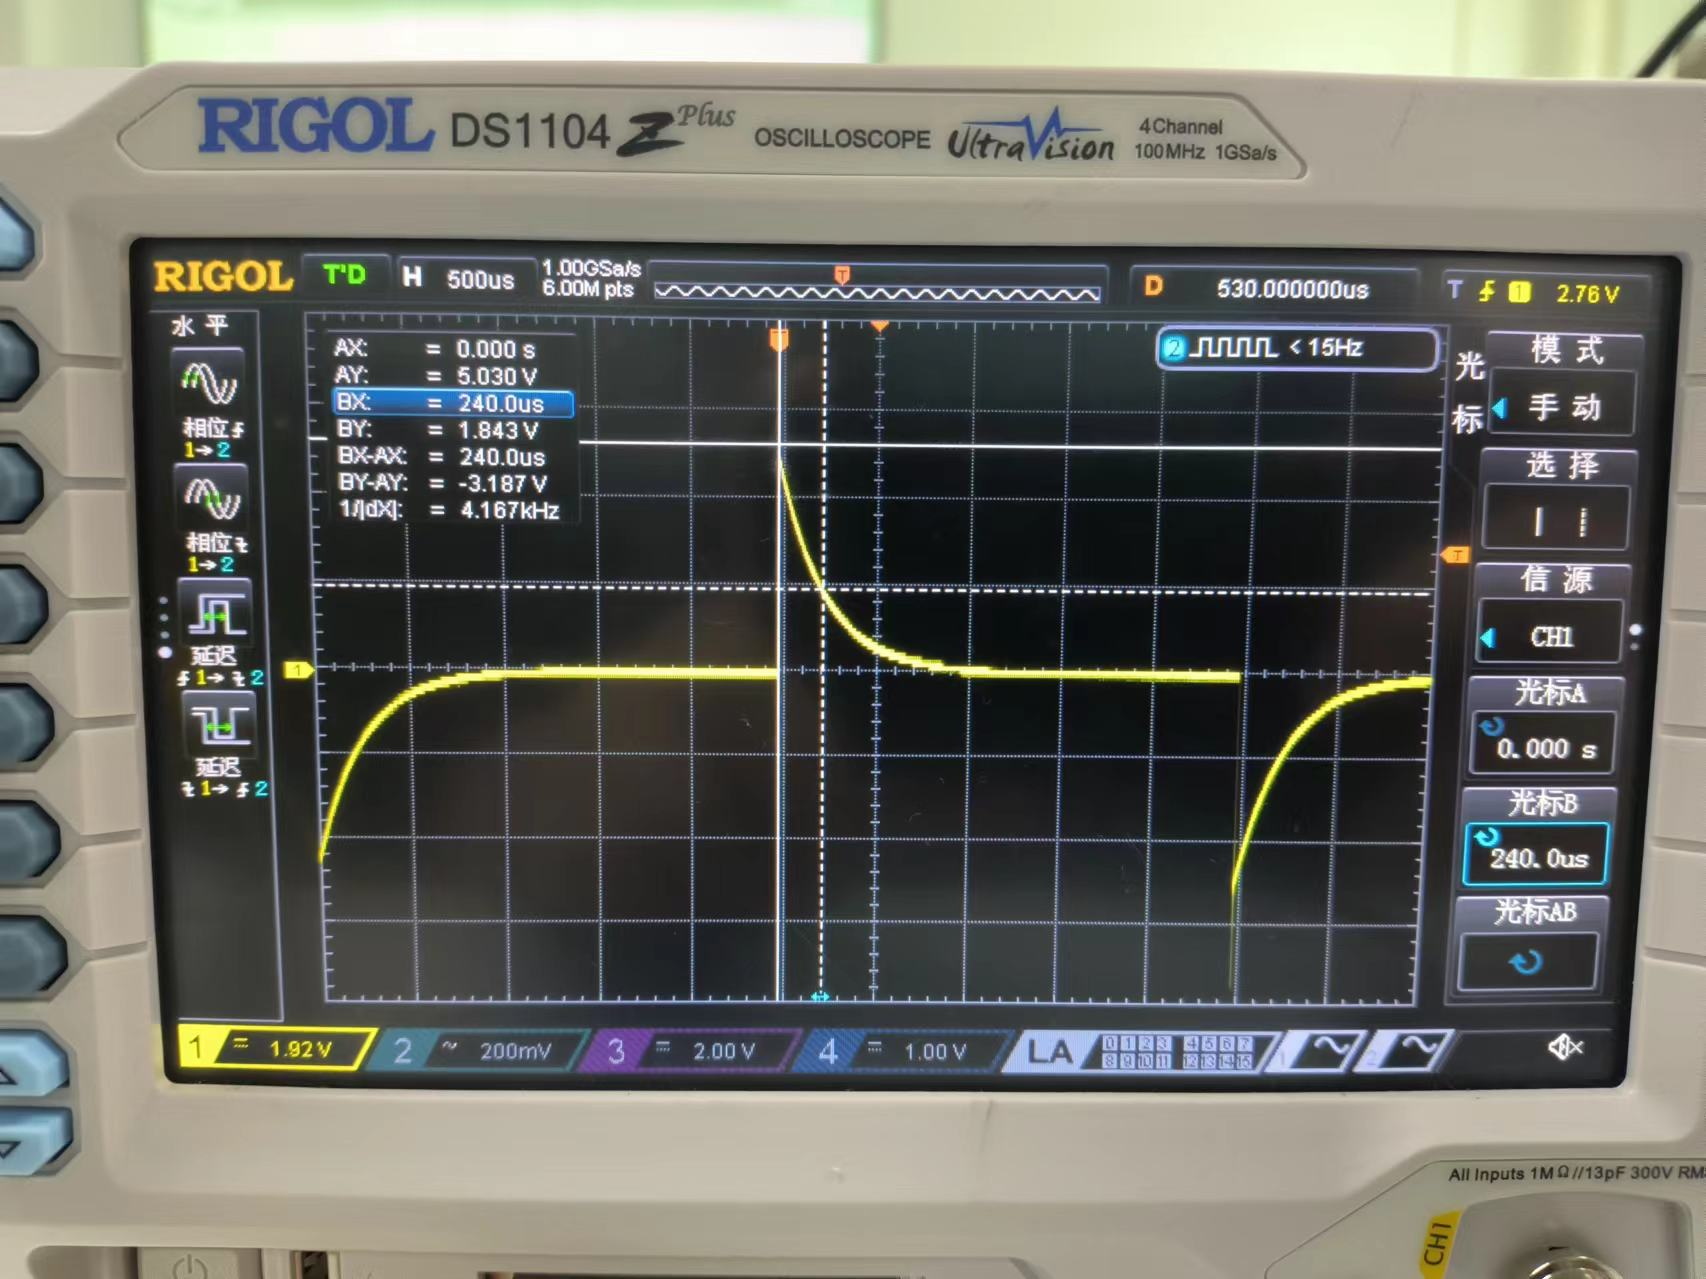
\includegraphics[width=0.35\textwidth]{graph2-11.jpg}\label{fig:graph2-11}}
			\quad
			\subfloat[$\tau=0.51ms$]
			{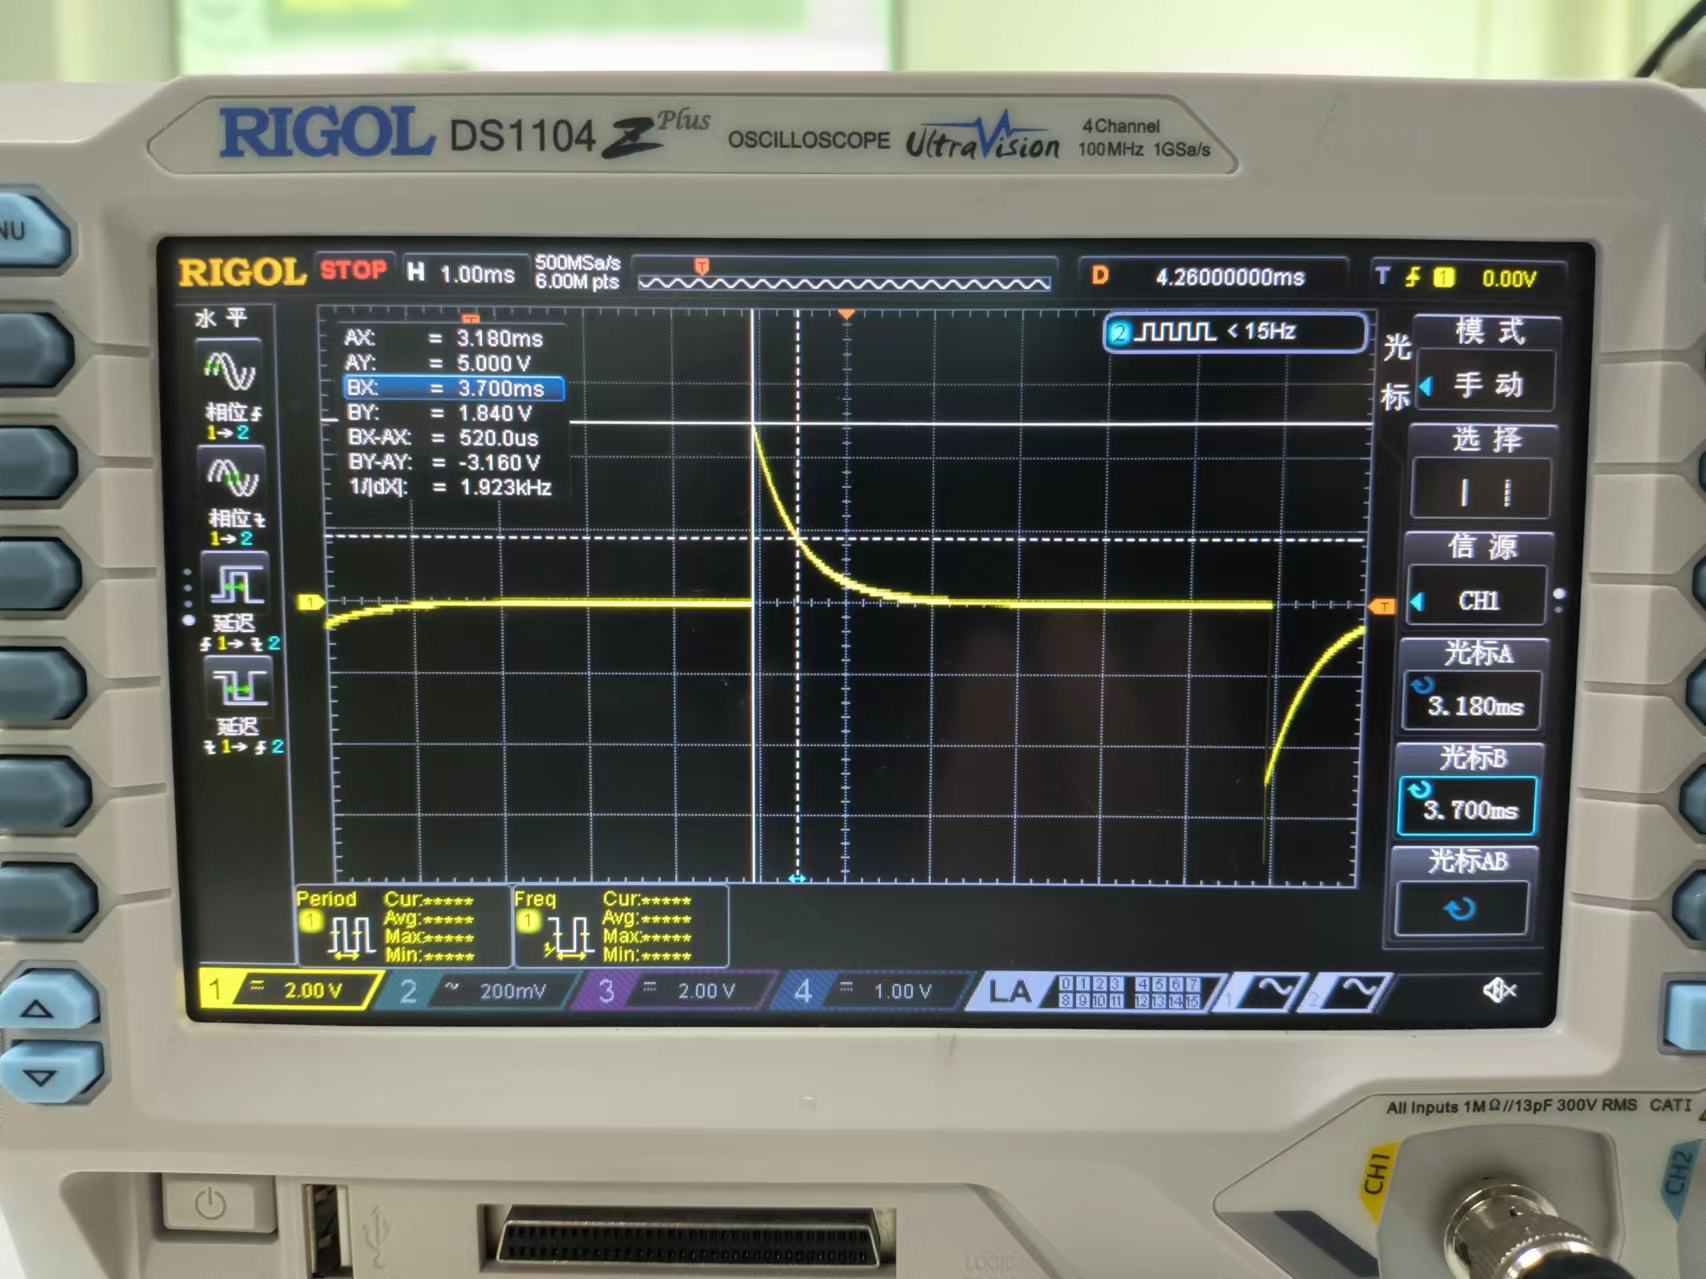
\includegraphics[width=0.35\textwidth]{graph2-12.jpg}\label{fig:graph2-12}}
			\quad
			\caption{RC微分电路波形图}
			\label{fig:graph2-1}
		\end{figure}

		RL微分电路,$L=100mH$,当$R=3k\Omega$时,输出波形如\cref{fig:graph2-21}所示;当$R=5.1k\Omega$时,输出波形如\cref{fig:graph2-22}所示。

		\begin{figure}[htbp]
			\centering
			\subfloat[$\tau=0.033ms$]
			{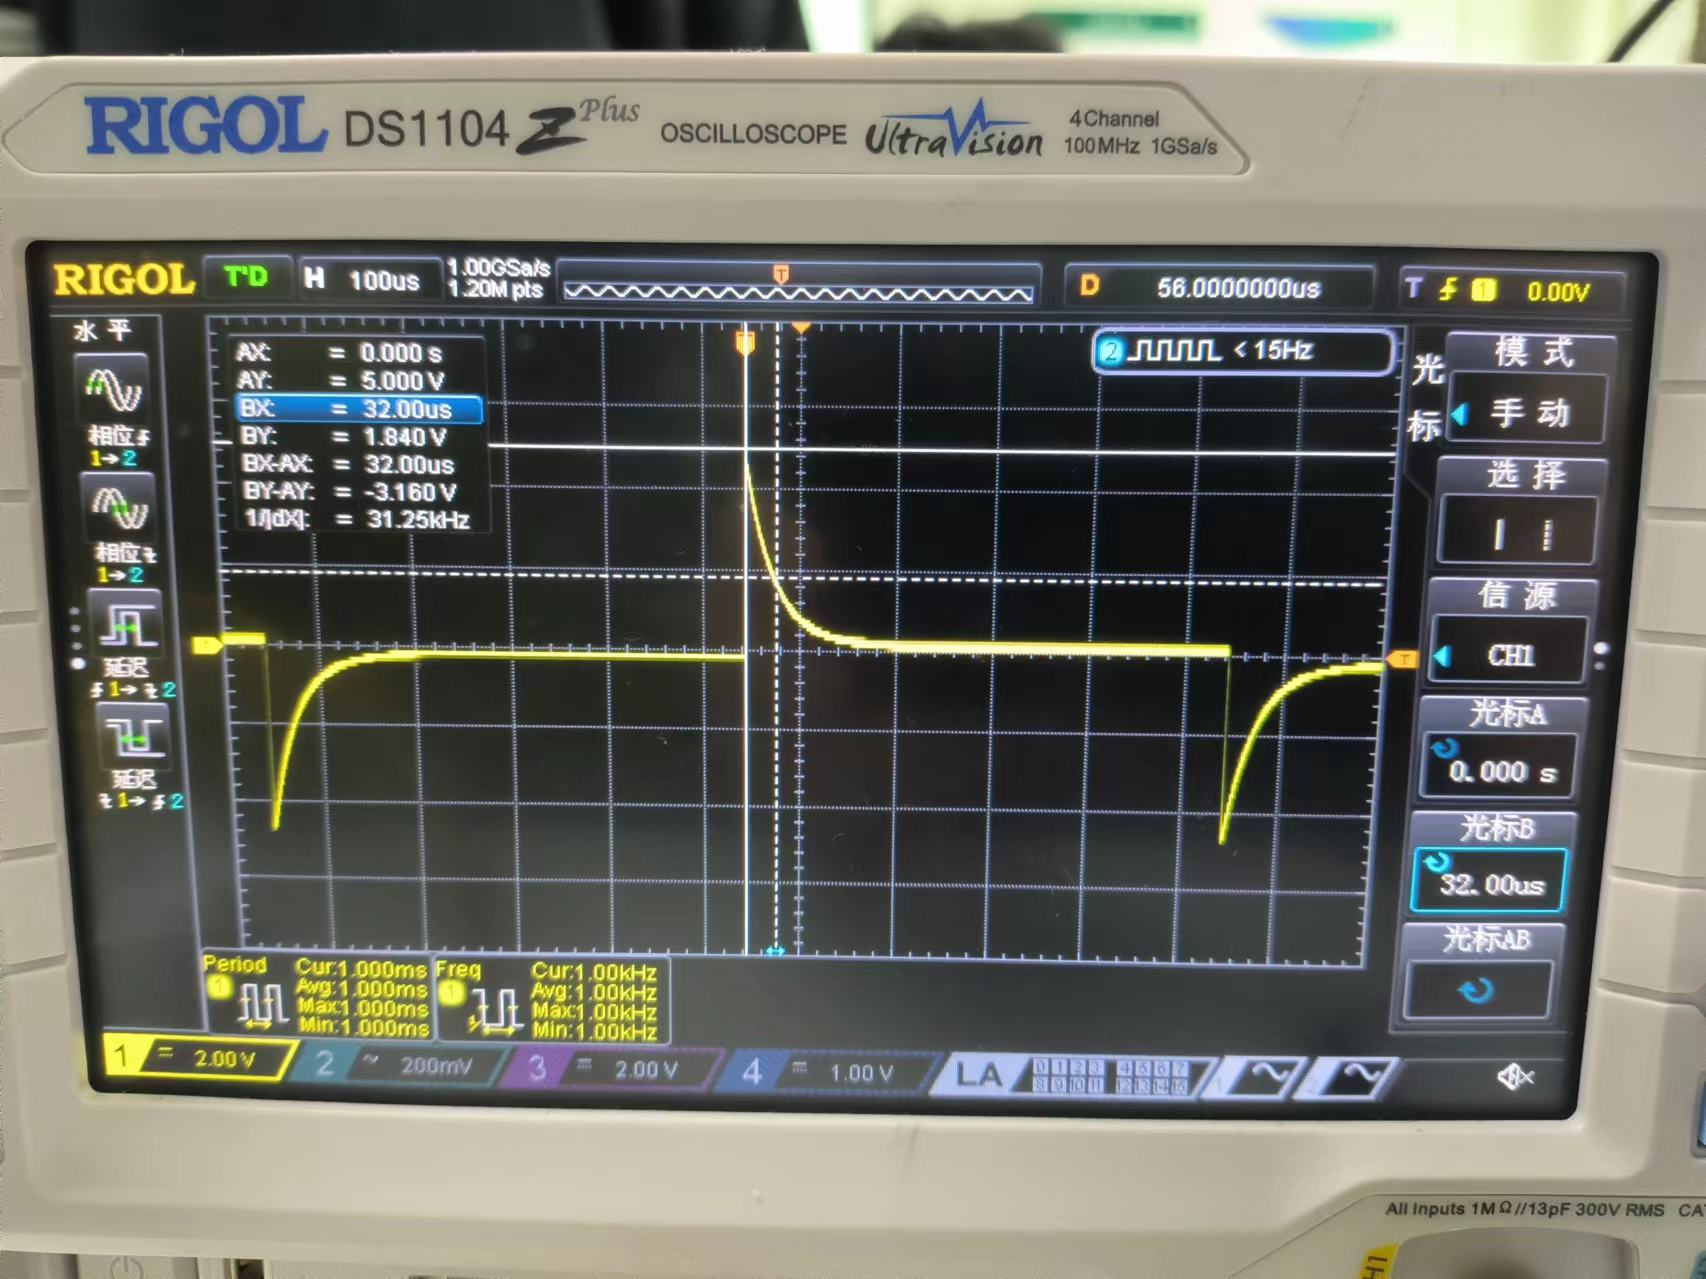
\includegraphics[width=0.35\textwidth]{graph2-21.jpg}\label{fig:graph2-21}}
			\quad
			\subfloat[$\tau=0.0196ms$]
			{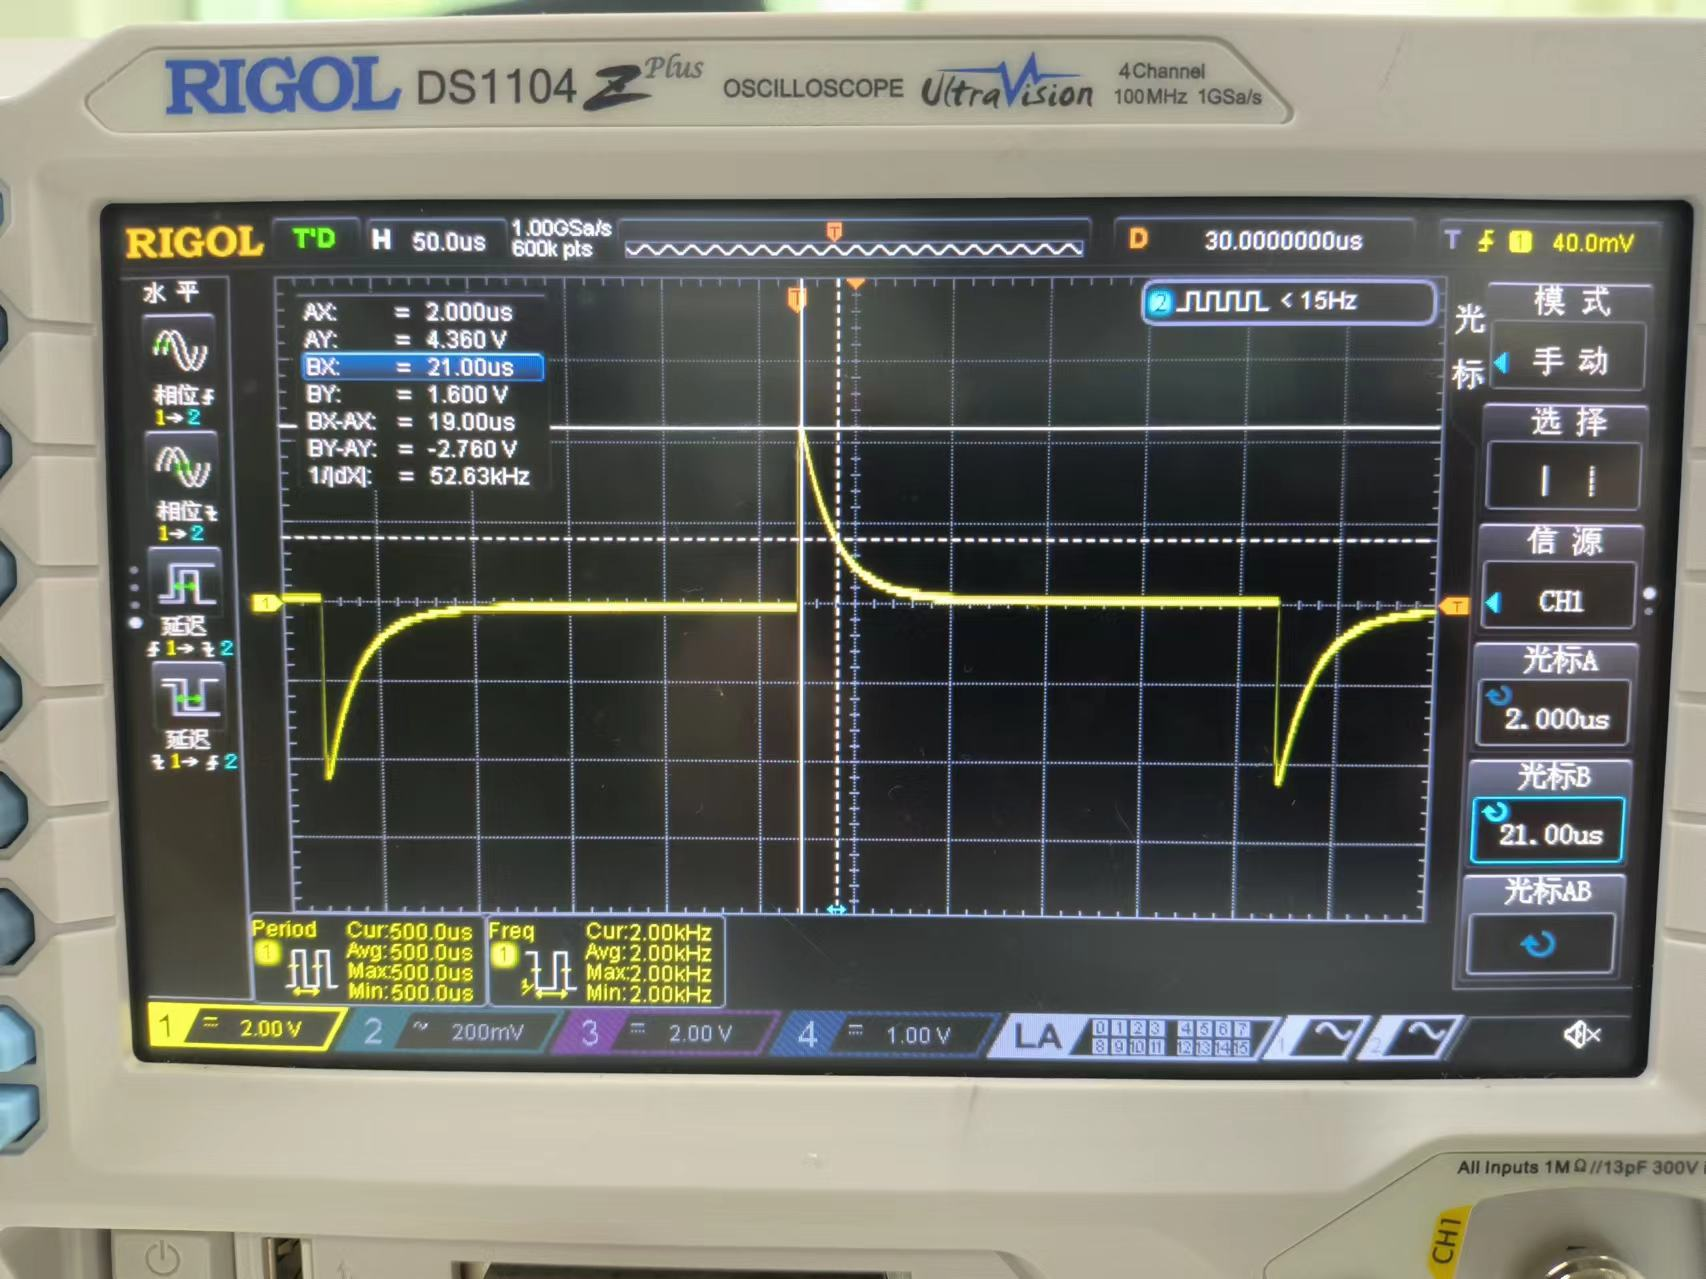
\includegraphics[width=0.35\textwidth]{graph2-22.jpg}\label{fig:graph2-22}}
			\quad
			\caption{RL微分电路波形图}
			\label{fig:graph2-2}
		\end{figure}

		RC积分电路,$C=10\mu F$,当$R=3k\Omega$时,输出波形如\cref{fig:graph2-31}所示;当$R=5.1k\Omega$时,输出波形如\cref{fig:graph2-32}所示。

		\begin{figure}[htbp]
			\centering
			\subfloat[$\tau=0.3ms$]
			{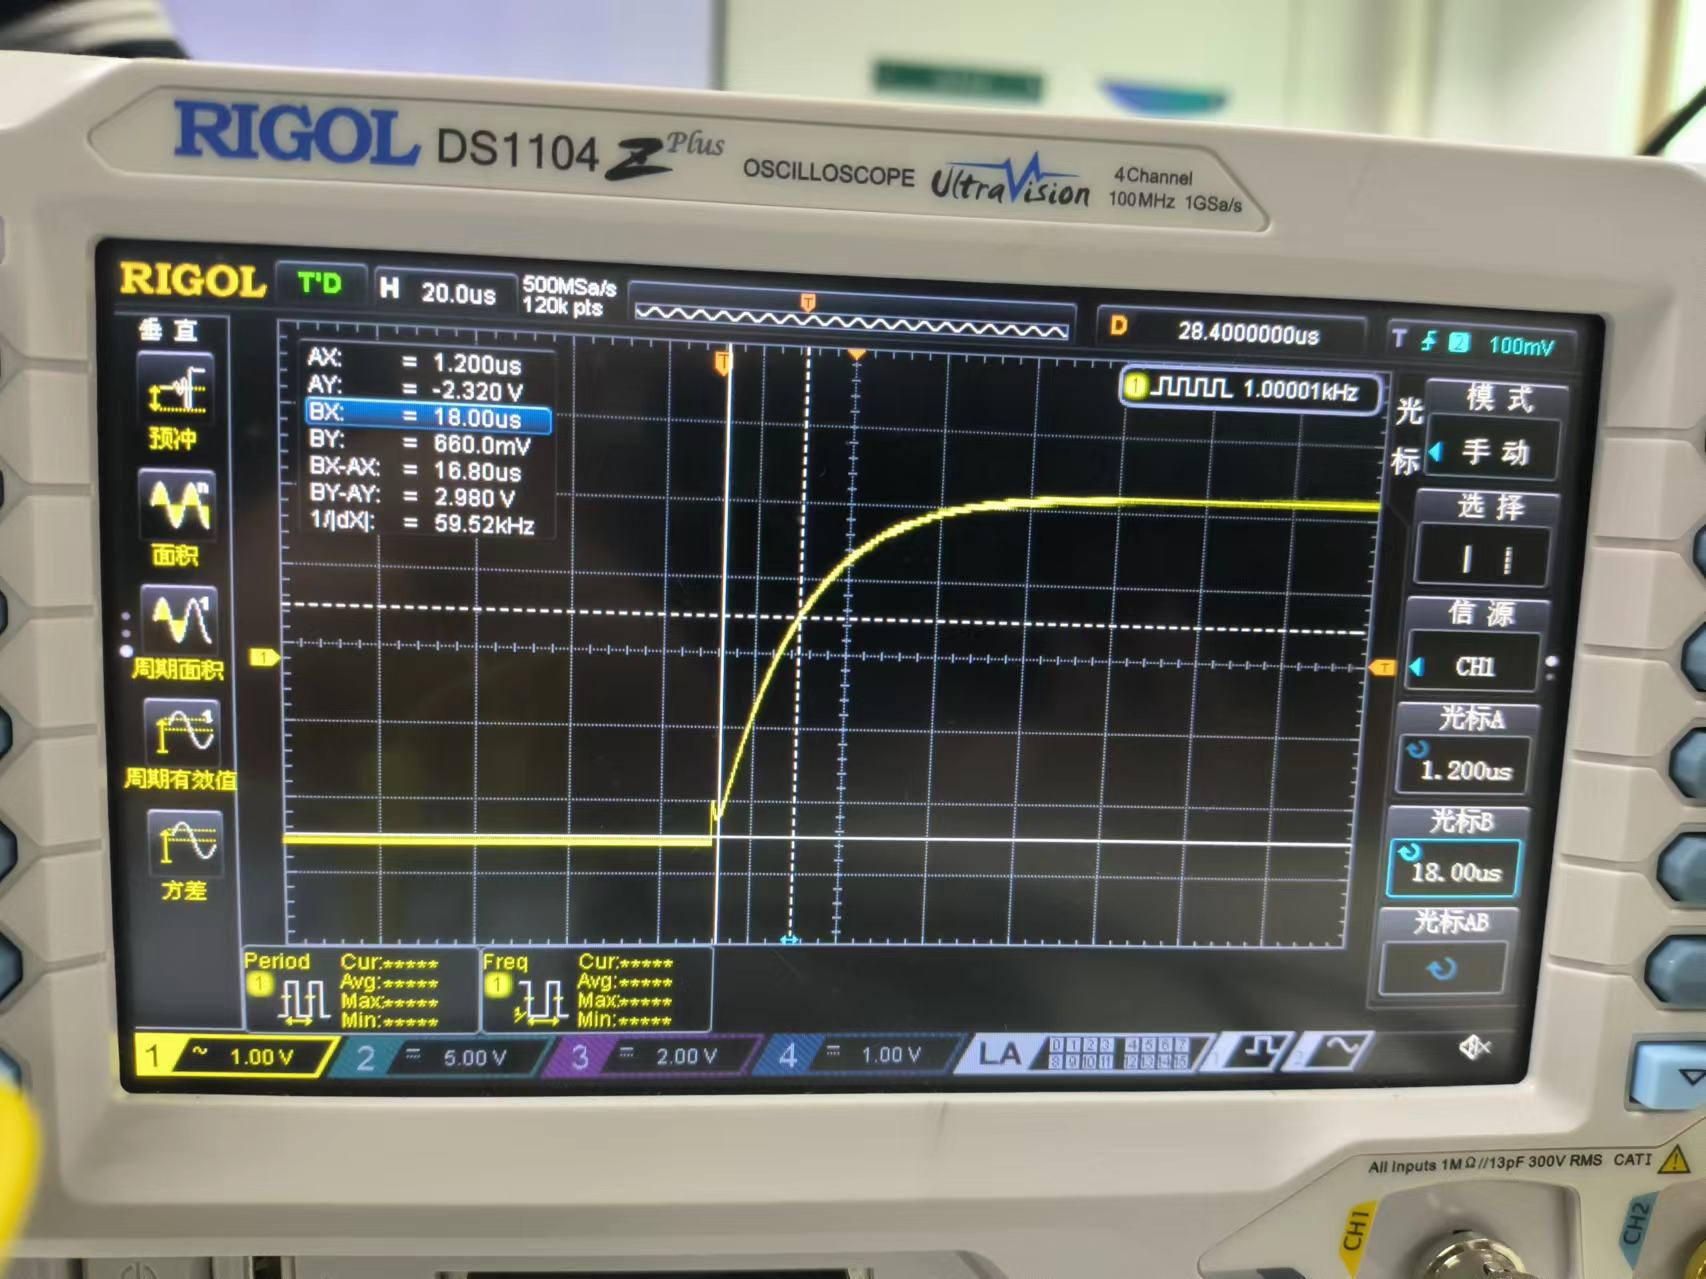
\includegraphics[width=0.35\textwidth]{graph2-31.jpg}\label{fig:graph2-31}}
			\quad
			\subfloat[$\tau=0.51ms$]
			{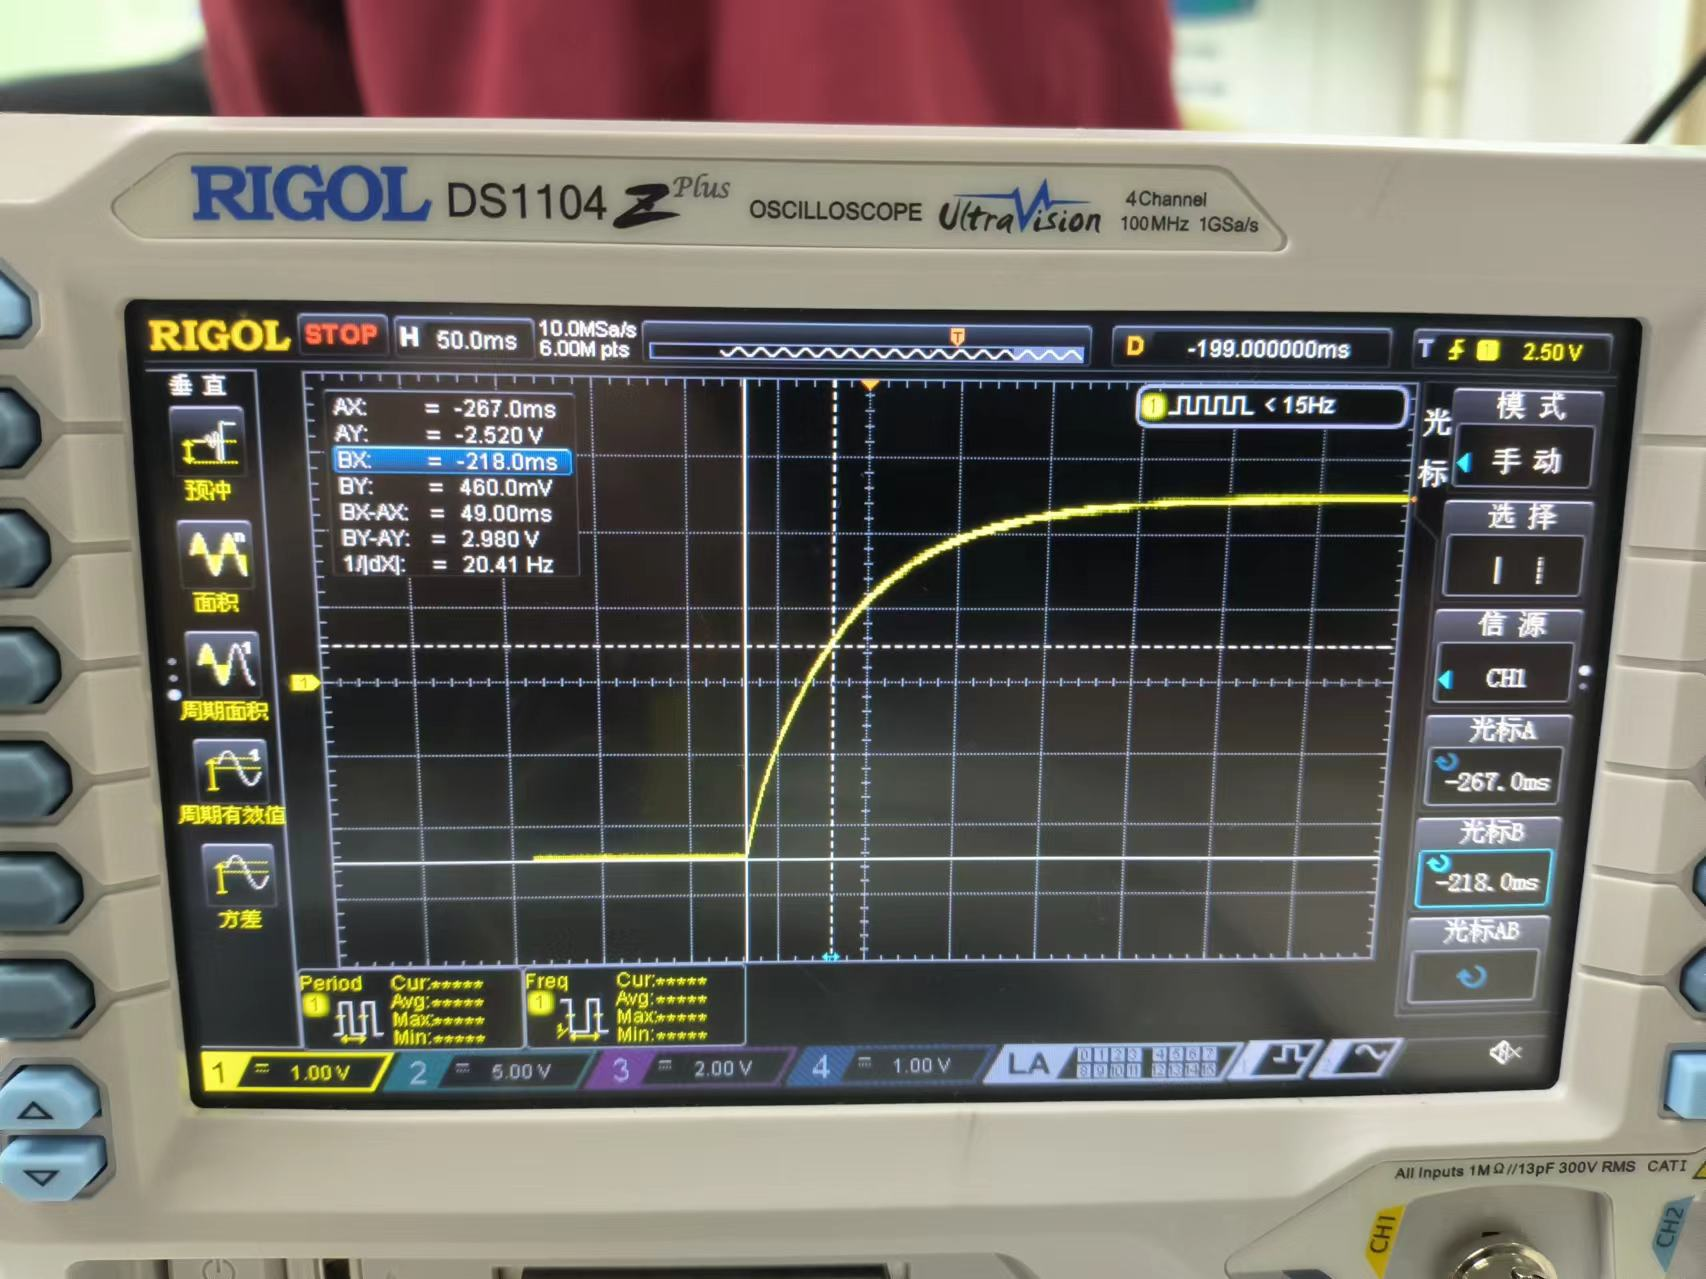
\includegraphics[width=0.35\textwidth]{graph2-32.jpg}\label{fig:graph2-32}}
			\quad
			\caption{RC积分电路波形图}
			\label{fig:graph2-3}
		\end{figure}
		
		RL积分电路,$L=100mH$,当$R=2.4k\Omega$时,输出波形如\cref{fig:graph2-41}所示;当$R=5.1k\Omega$时,输出波形如\cref{fig:graph2-42}所示。

		\begin{figure}[htbp]
			\centering
			\subfloat[$\tau=0.0416ms$]
			{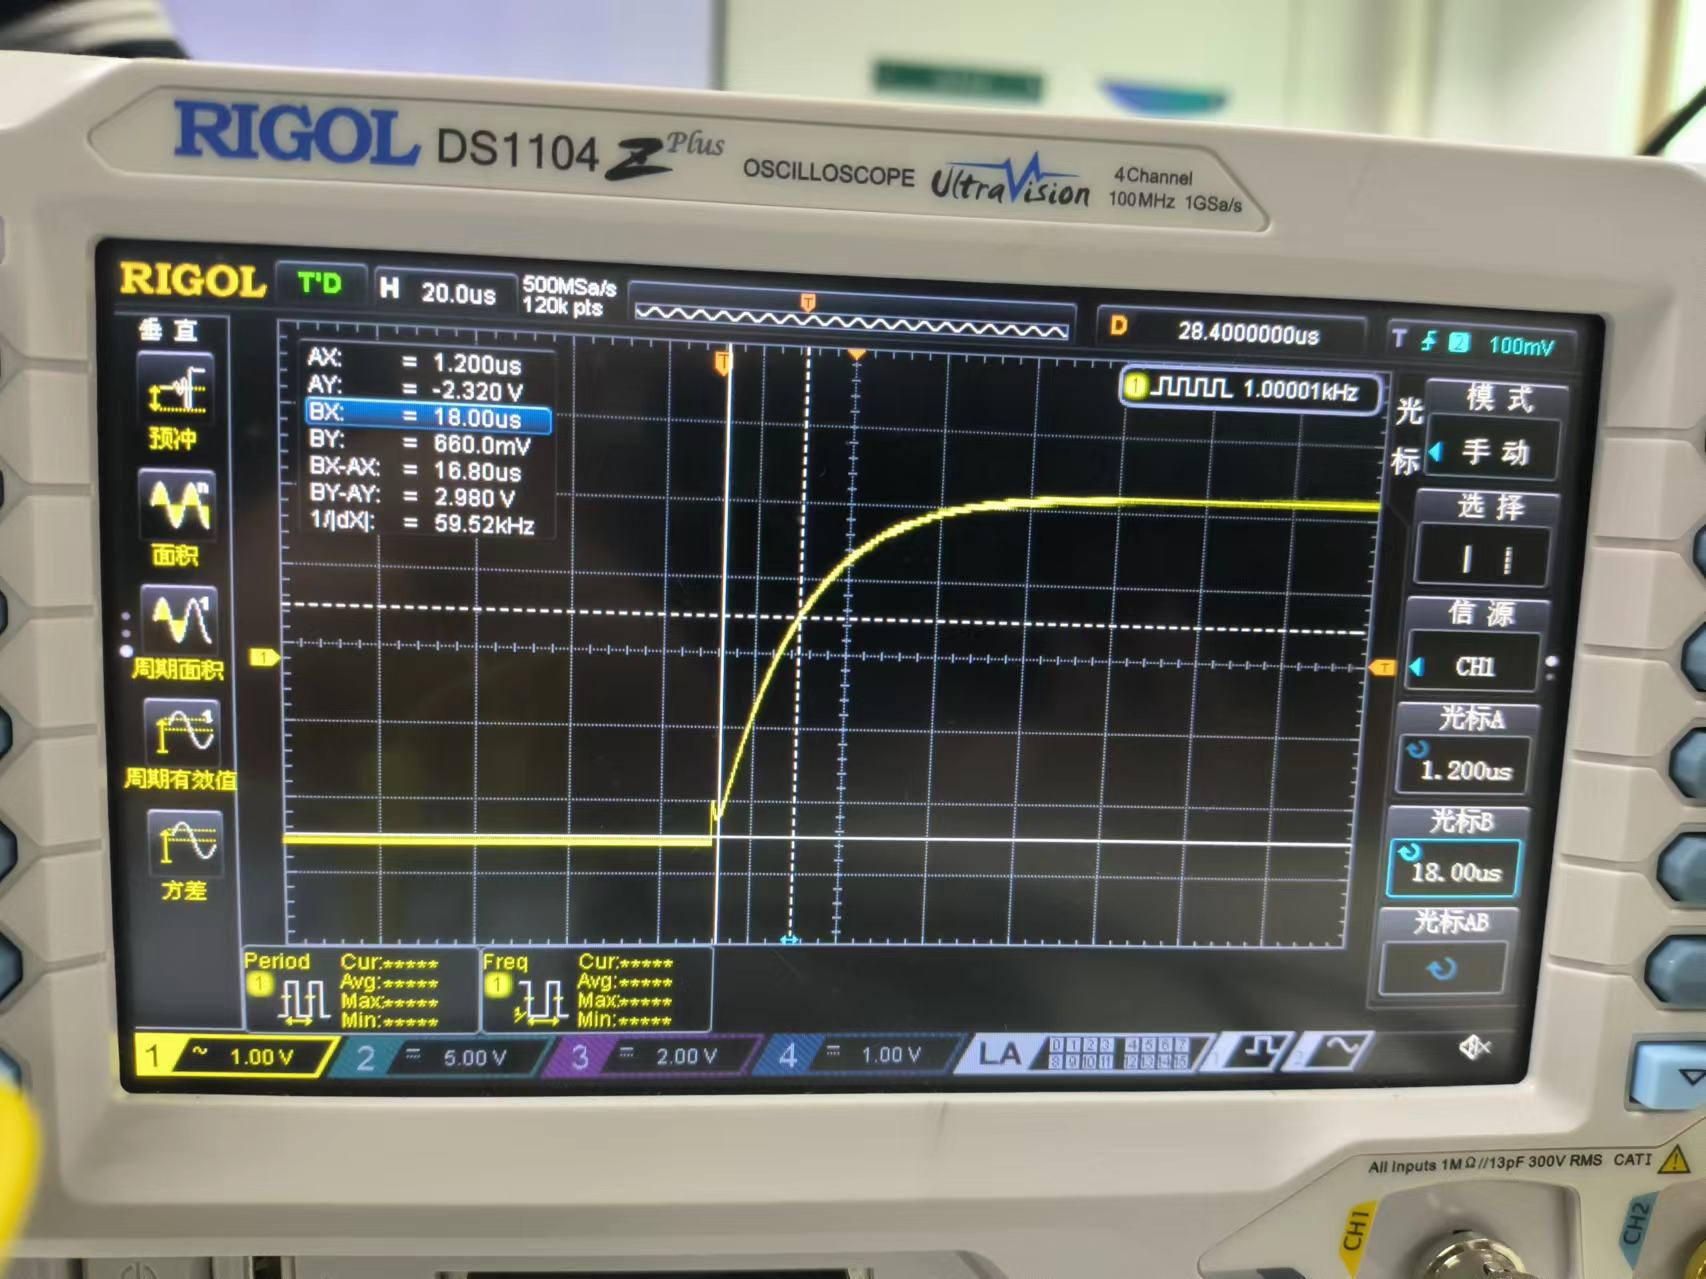
\includegraphics[width=0.35\textwidth]{graph2-41.jpg}\label{fig:graph2-41}}
			\quad
			\subfloat[$\tau=0.0196ms$]
			{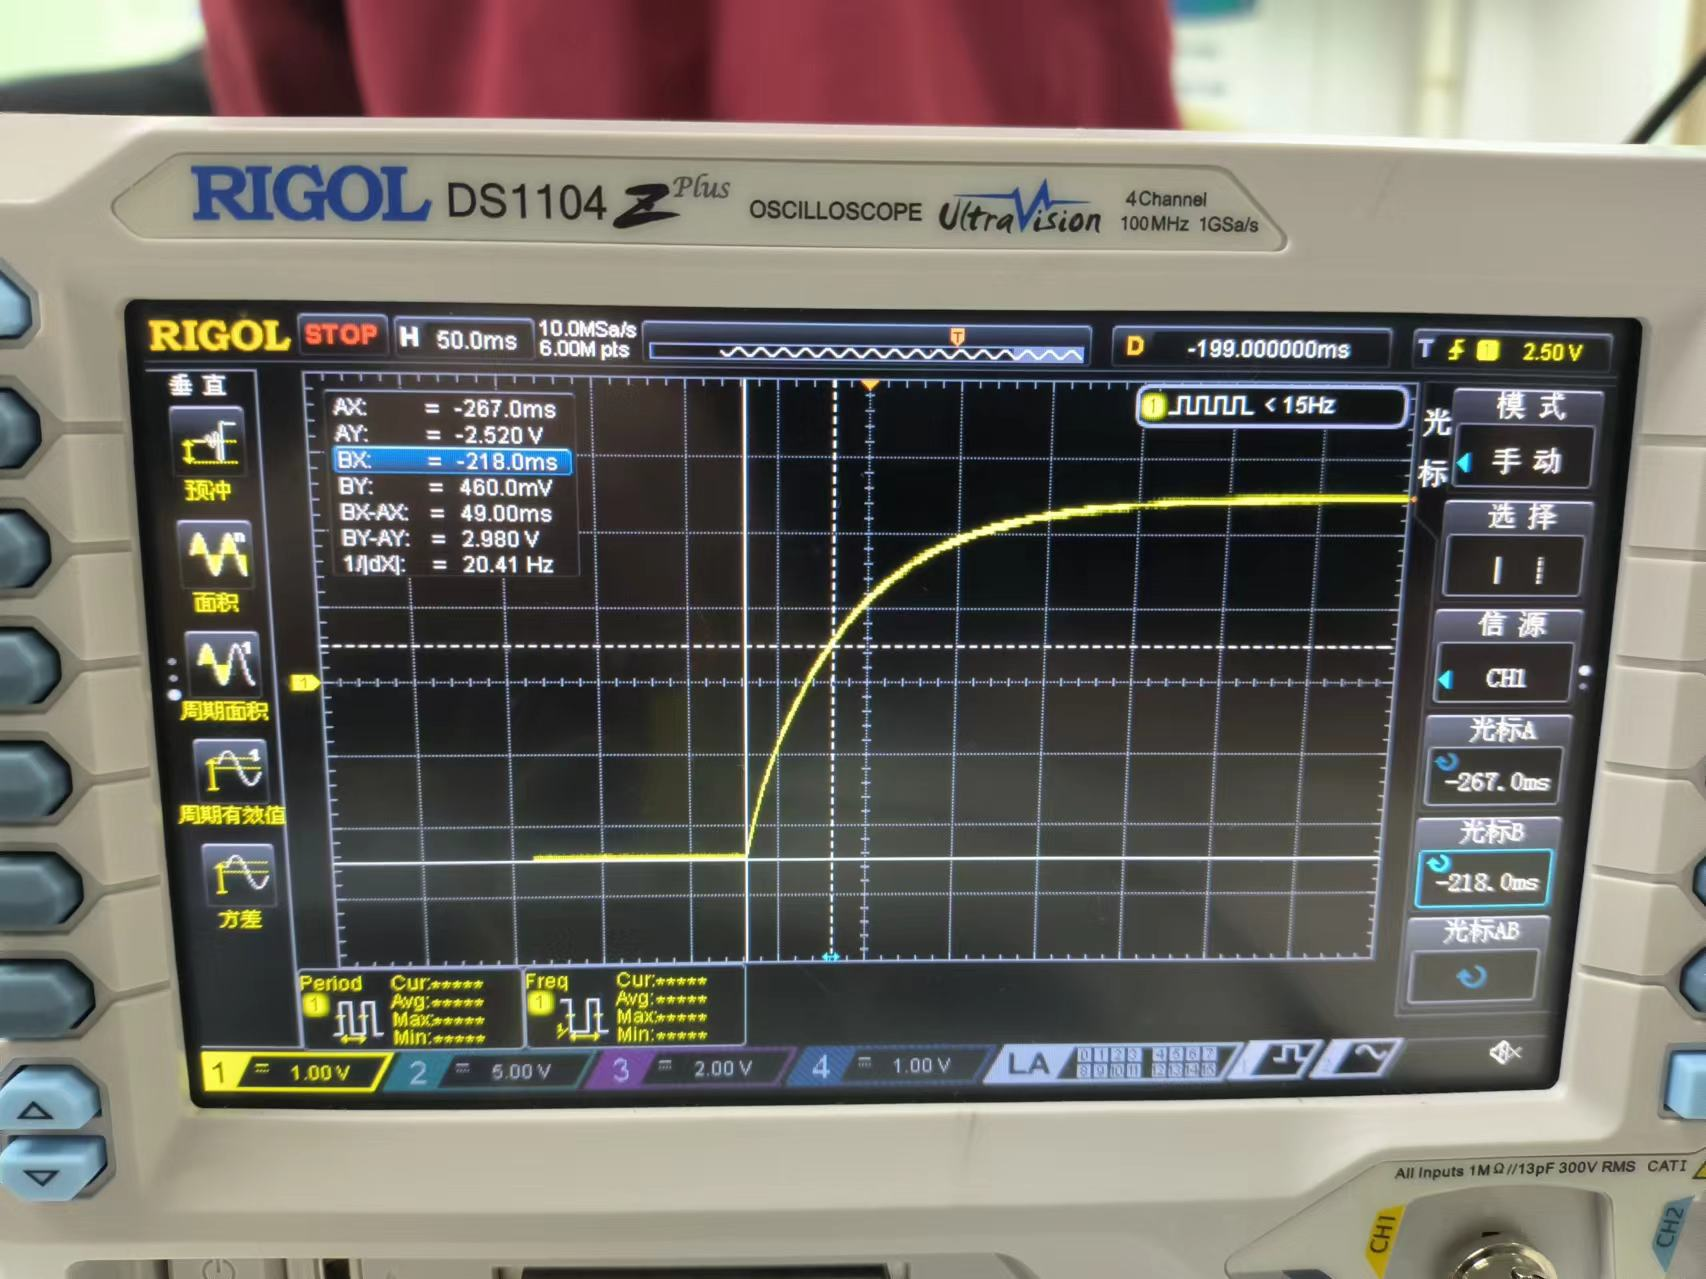
\includegraphics[width=0.35\textwidth]{graph2-42.jpg}\label{fig:graph2-42}}
			\quad
			\caption{RL积分电路波形图}
			\label{fig:graph2-4}
		\end{figure}

		RC电路三角波型和RL电路三角波型如图\cref{fig:graph2-5}所示

		\begin{figure}[htbp]
			\centering
			\subfloat[RC电路]
			{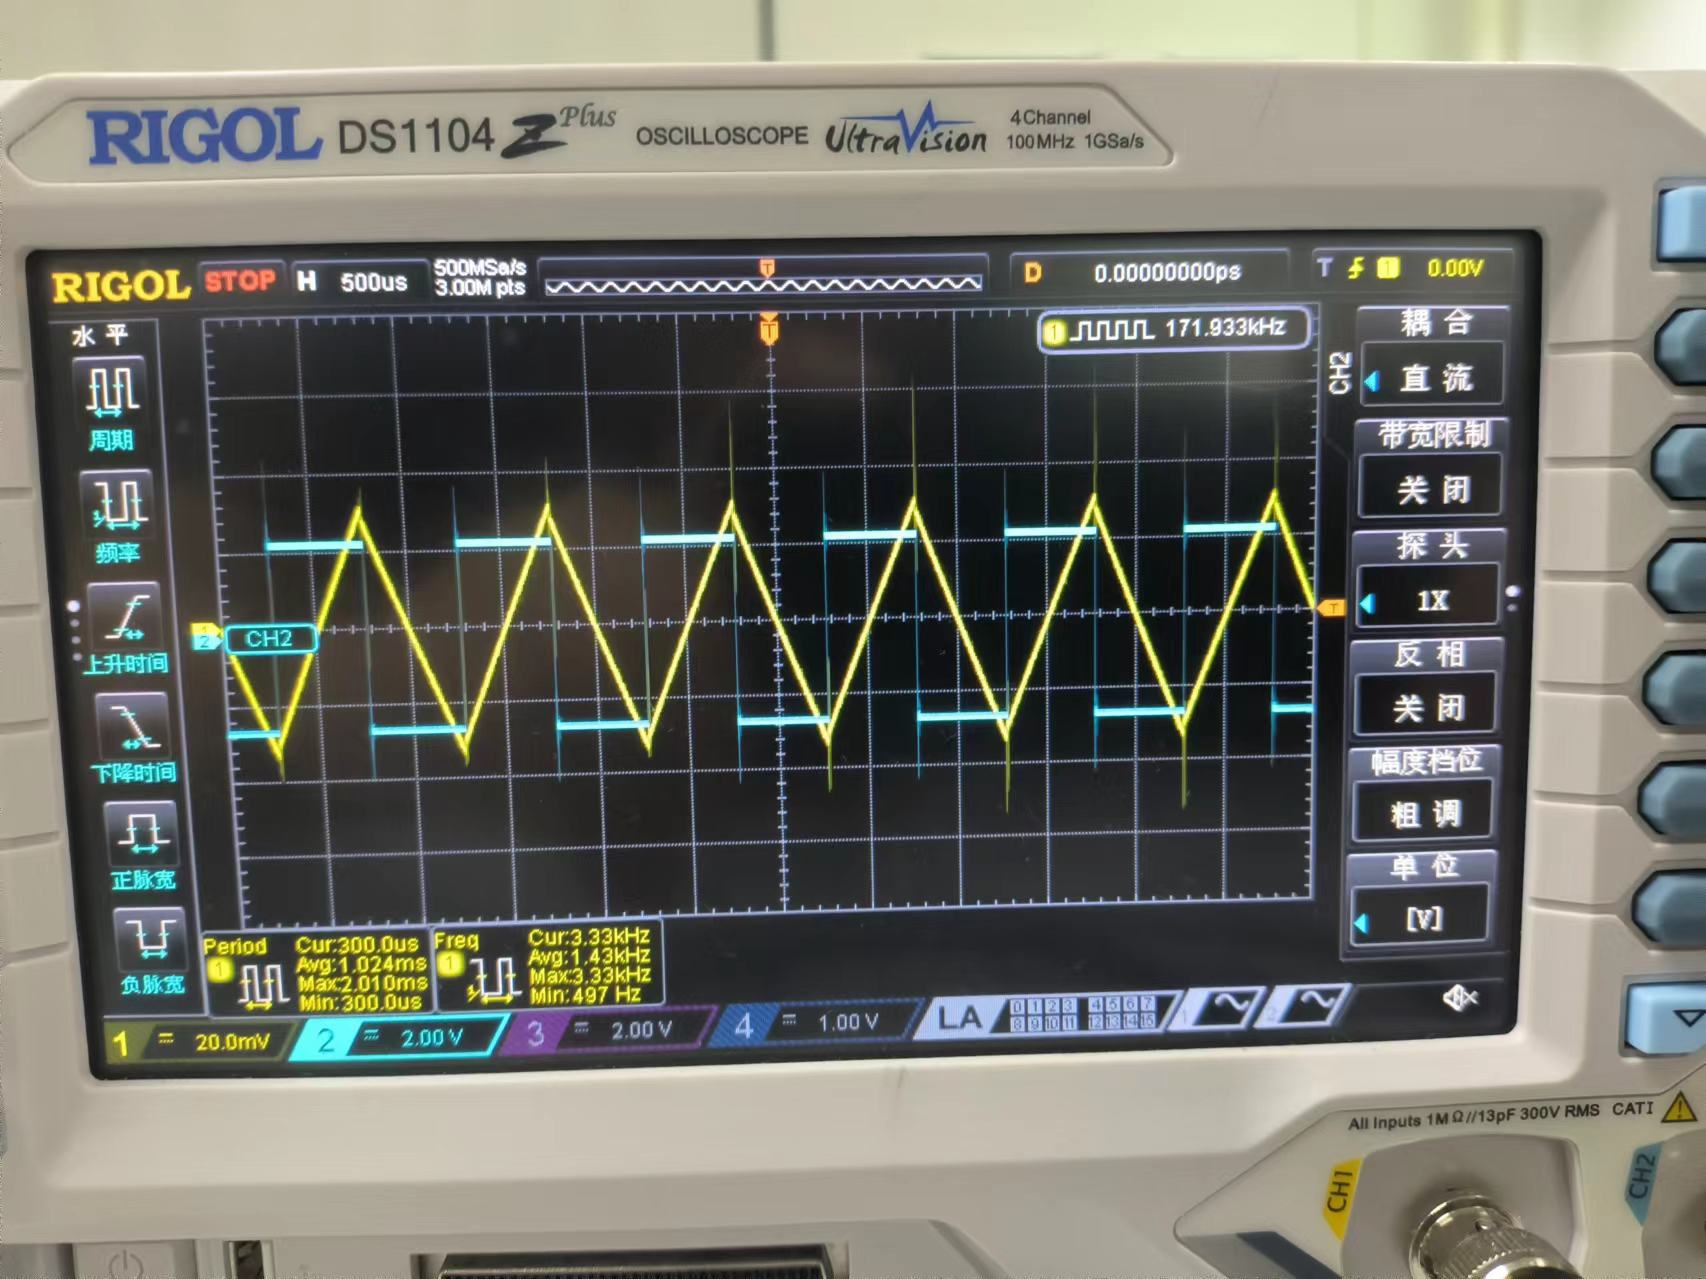
\includegraphics[width=0.35\textwidth]{graph2-51.jpg}\label{fig:graph2-51}}
			\quad
			\subfloat[RL电路]
			{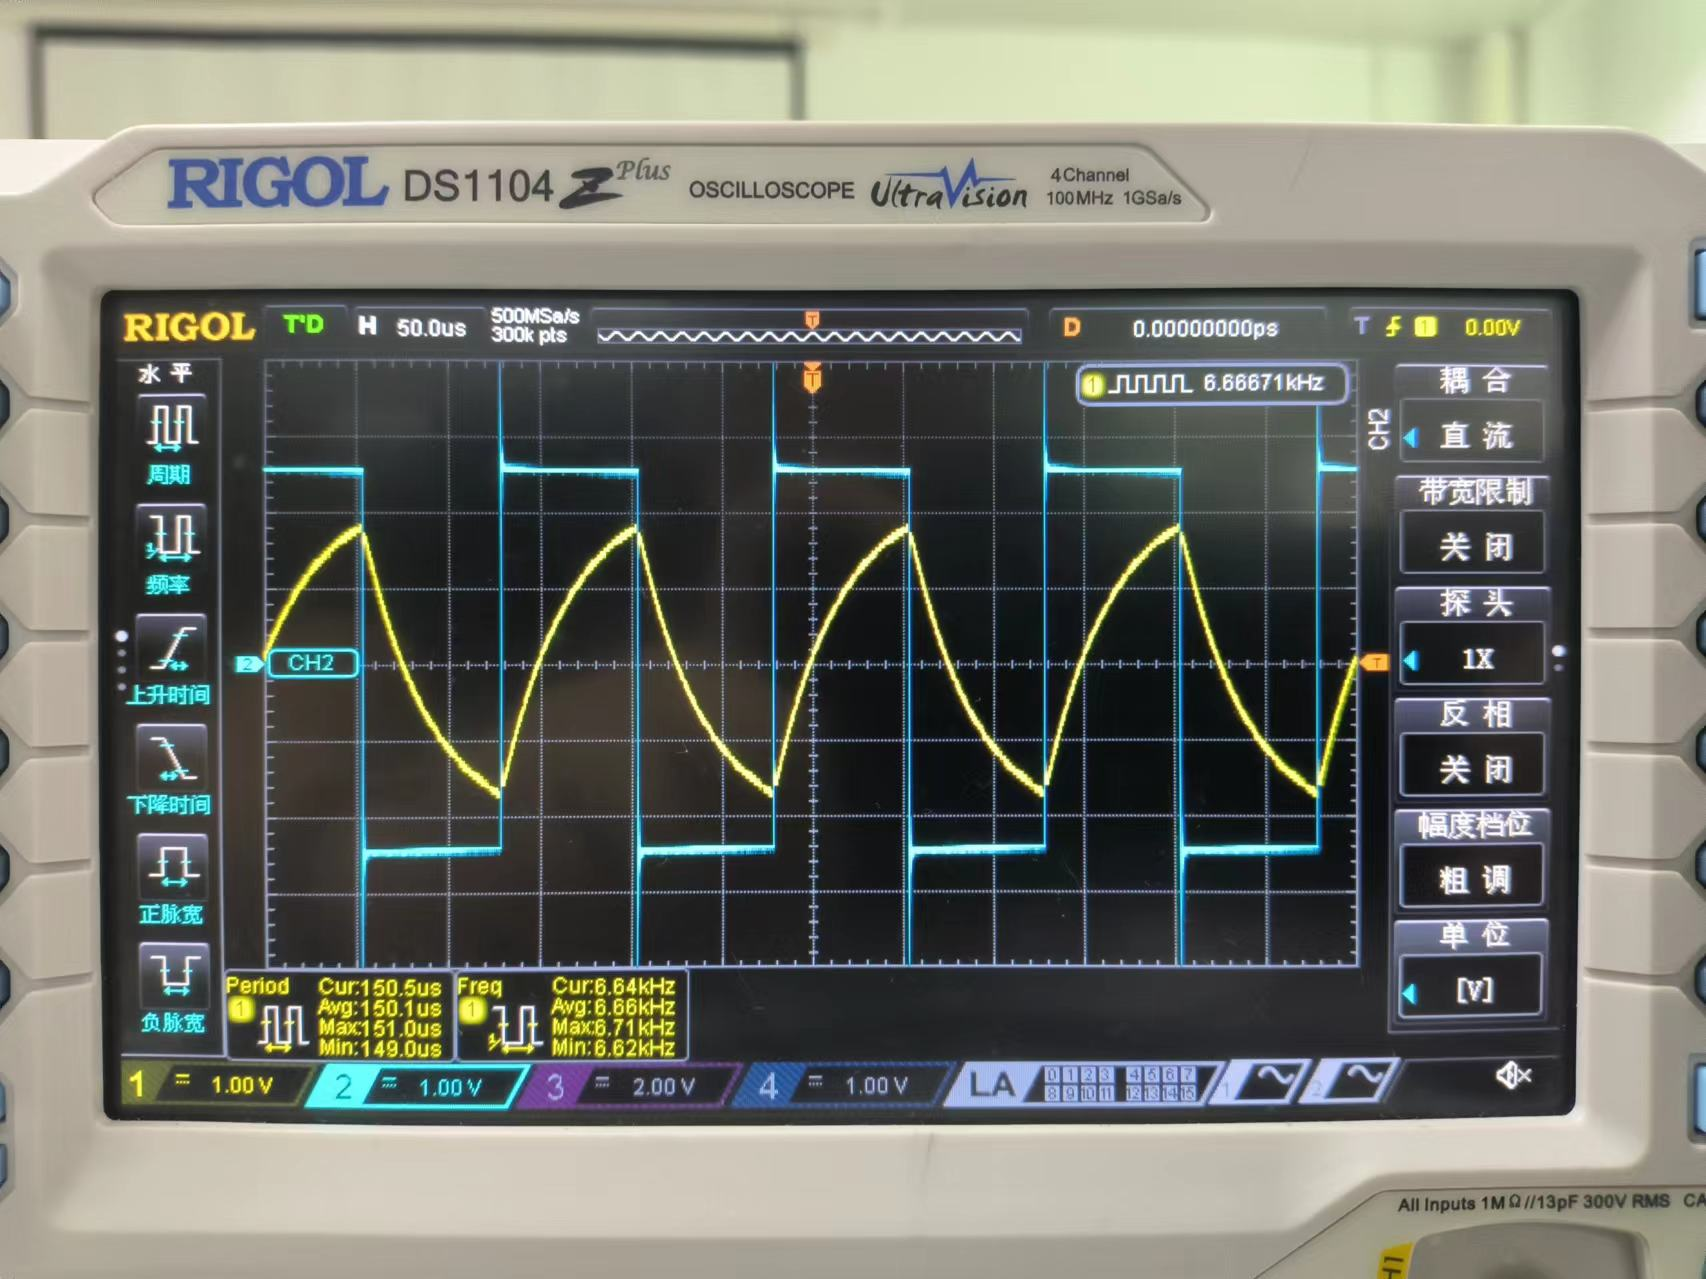
\includegraphics[width=0.35\textwidth]{graph2-52.jpg}\label{fig:graph2-52}}
			\quad
			\caption{RC电路和RL电路三角波}
			\label{fig:graph2-5}
		\end{figure}
		
		\item 时间常数测量结果如\cref{tab:tab1}所示。
		
		\begin{table}[h]
			\centering
			\caption{电路时间常数测量值}
			\label{tab:tab1}
			\begin{tabular}{|c|c|c|c|c|}
				\hline
				电路 & AX & BX & 时间常数测量值 & 单位 \\
				\hline
				RC微分 2.4kΩ & 0.00 & 240.00 & 240.00 & $\mu s$ \\
				RC微分 5.1kΩ & 3.18 & 3.70 & 0.52 & ms \\
				RL微分 3kΩ & 0.00 & 32.00 & 32.00 & $\mu s$ \\
				RL微分 5.1kΩ & 2.00 & 21.00 & 19.00 & $\mu s$ \\
				RL积分 2.4kΩ & 0.00 & 37.00 & 37.00 & $\mu s$ \\
				RL积分 5.1kΩ & 1.20 & 18.00 & 16.80 & $\mu s$ \\
				RC积分 3kΩ & -155.00 & -127.00 & 28.00 & ms \\
				RC积分 5.1kΩ & -267.00 & -218.00 & 49.00 & ms \\
				\hline
			\end{tabular}
		\end{table}					
			
	\end{enumerate}
	
	% ---
	
	% 原始数据
	\clearpage
	\subsection{原始数据记录}
	实验记录本上的原始数据见\cref{fig:figdata-1}、\cref{fig:figdata-2}(签字)。

		\begin{figure}[htbp]
			\centering
			\subfloat[原始数据1]
			{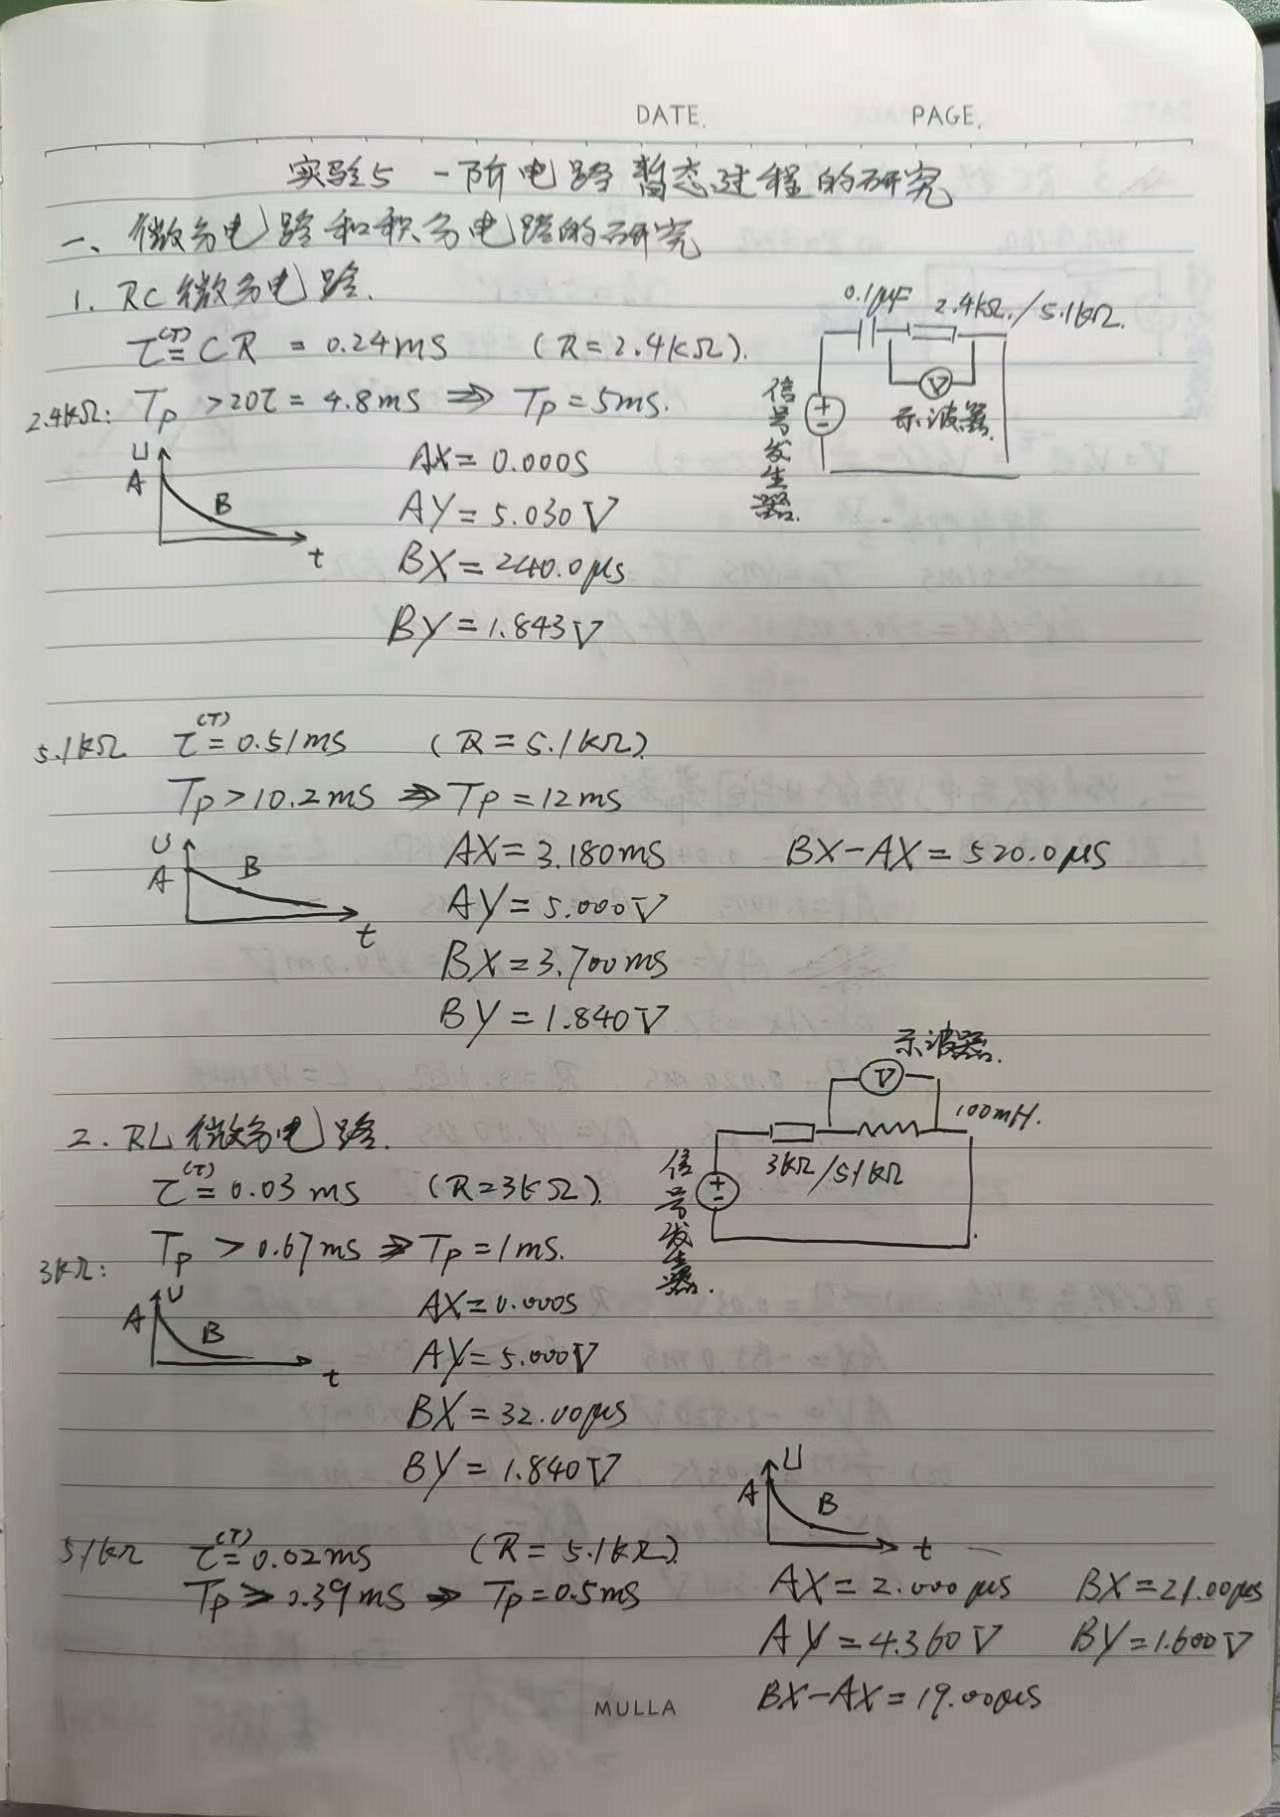
\includegraphics[width=0.4\textwidth]{ET1_5Gradata-1.jpg}\label{fig:figdata-1}}
			\quad
			\subfloat[原始数据2]
			{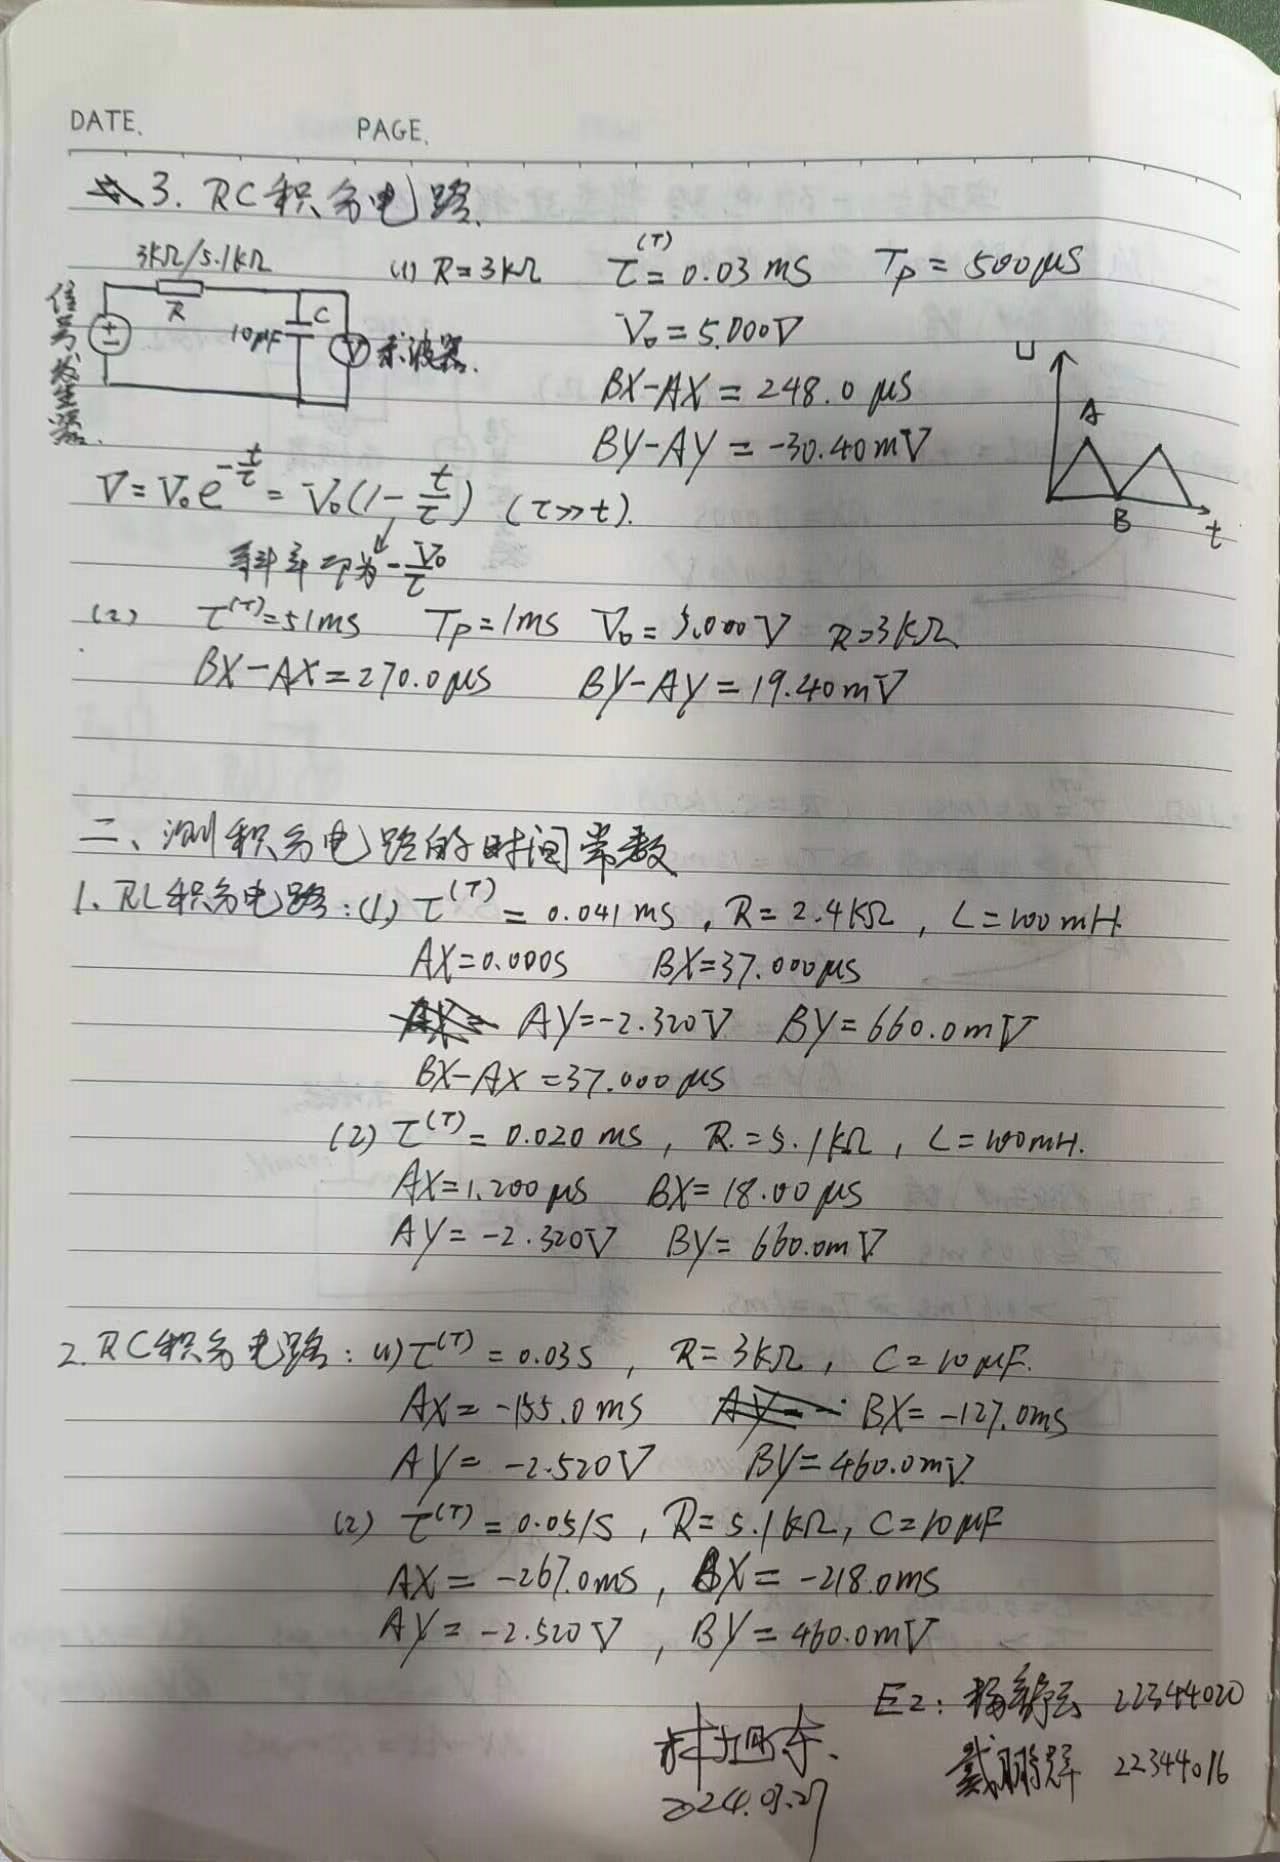
\includegraphics[width=0.4\textwidth]{ET1_5Gradata-2.jpg}\label{fig:figdata-2}}
			\quad
			\caption{实验原始数据}
			\label{fig:graph10}
		\end{figure}
	
	%实验台桌面整理见%\textbf{附件}部分(\cref{})。
	
	%其它原始数据见%\cref{}。
	% ---
	
	% 问题记录
	%\begin{enumerate}
	%	\item 
	%\end{enumerate}
	% ---
	
	
	
	% 分析与讨论	
	\clearpage
	
	% 顶栏
	\begin{table}
		\renewcommand\arraystretch{1.7}
		\begin{tabularx}{\textwidth}{|X|X|X|X|}
			\hline
			专业:& 物理学 &年级:& 2022级\\
			\hline
			姓名: & 戴鹏辉、杨舒云 & 学号:& 22344016、22344020\\
			\hline
			日期:& 2024/3/27 & 评分: &\\
			\hline
		\end{tabularx}
	\end{table}
	% ---
	
	% 小标题
	\section{ET1-5 一阶电路暂态过程的研究 \quad\heiti 分析与讨论}
	% ---
	
	% 数据处理
	\subsection{实验数据分析}
	
	%
	\subsubsection{关于输出波形的讨论}
	\begin{enumerate}
		\item 微分电路波形比对
		
		\begin{figure}[htbp]
			\centering
			\subfloat[$R=2400\Omega$]
			{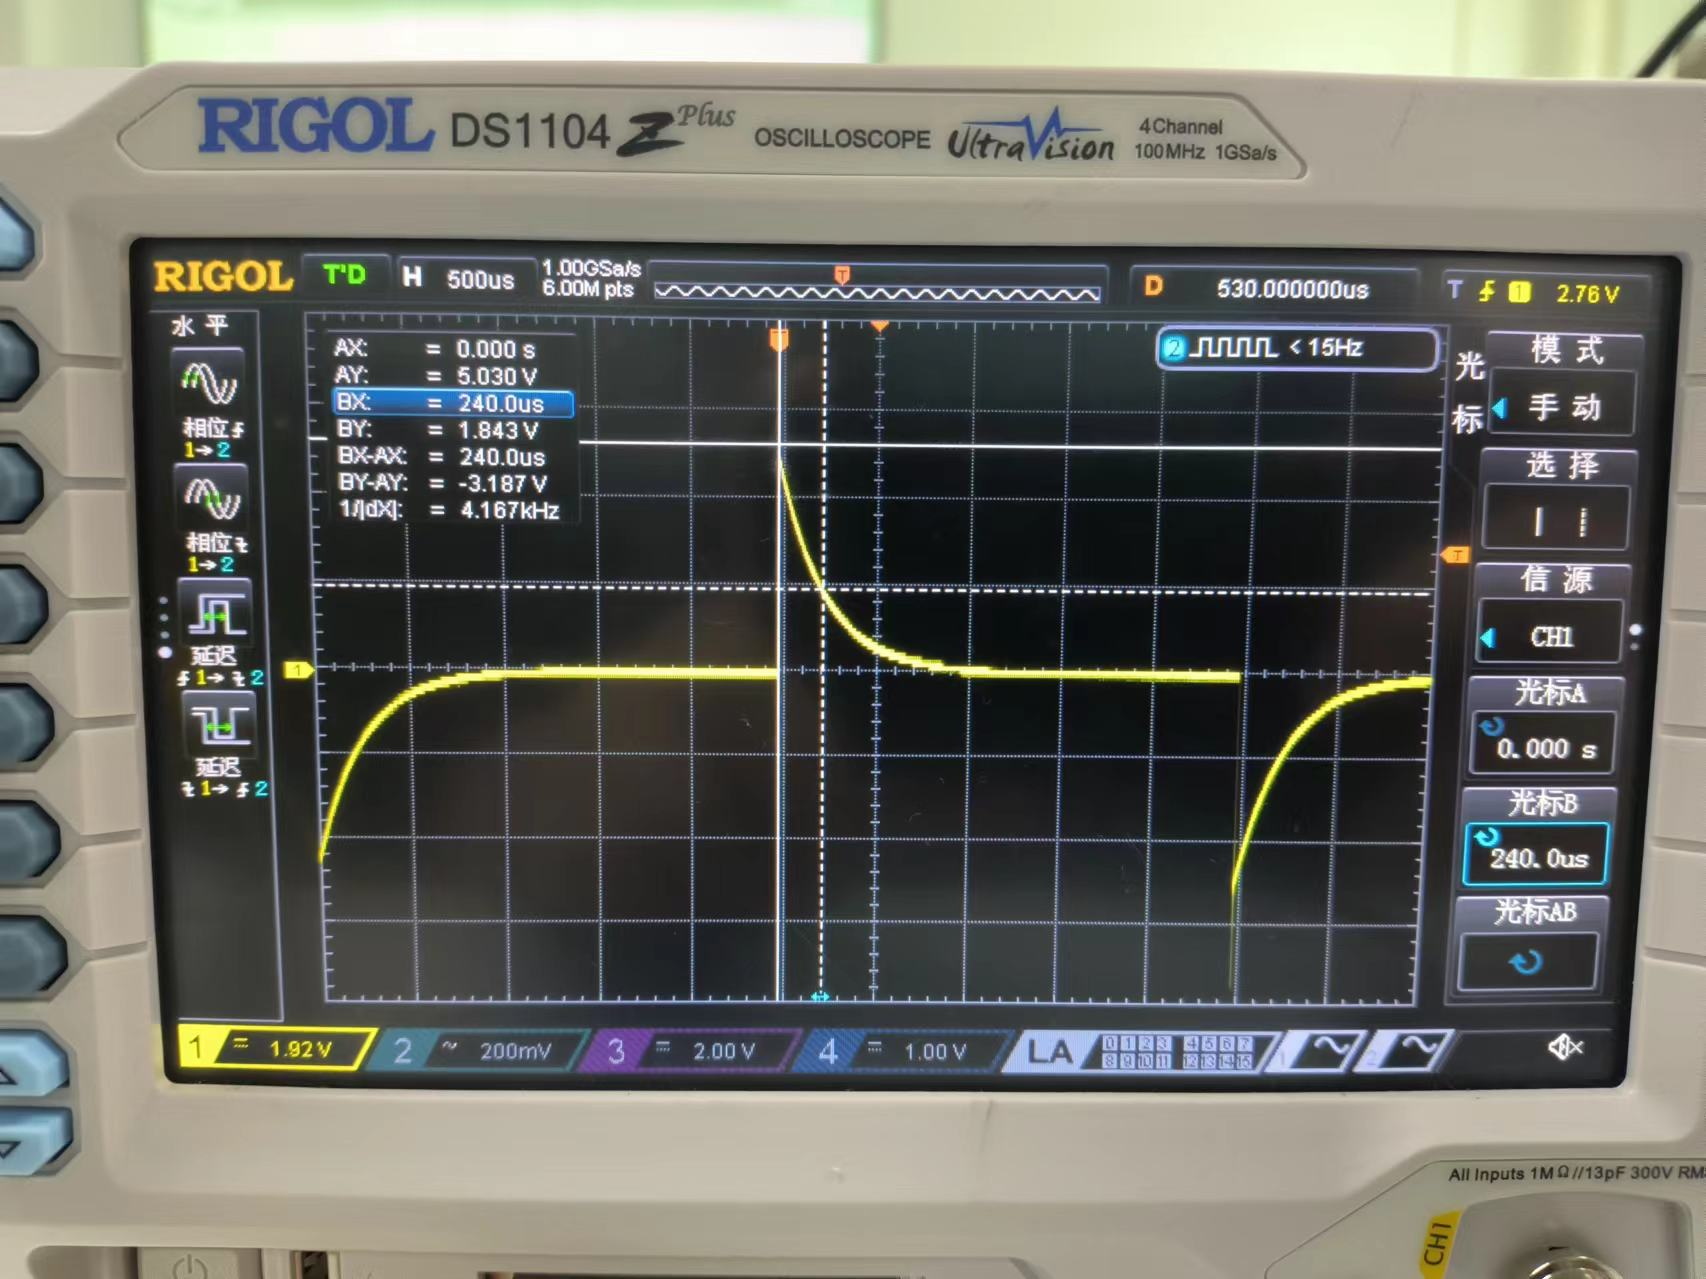
\includegraphics[width=0.35\textwidth]{graph2-11.jpg}\label{fig:graph3-1-1a}}
			\quad
			\subfloat[$R=5100\Omega$]
			{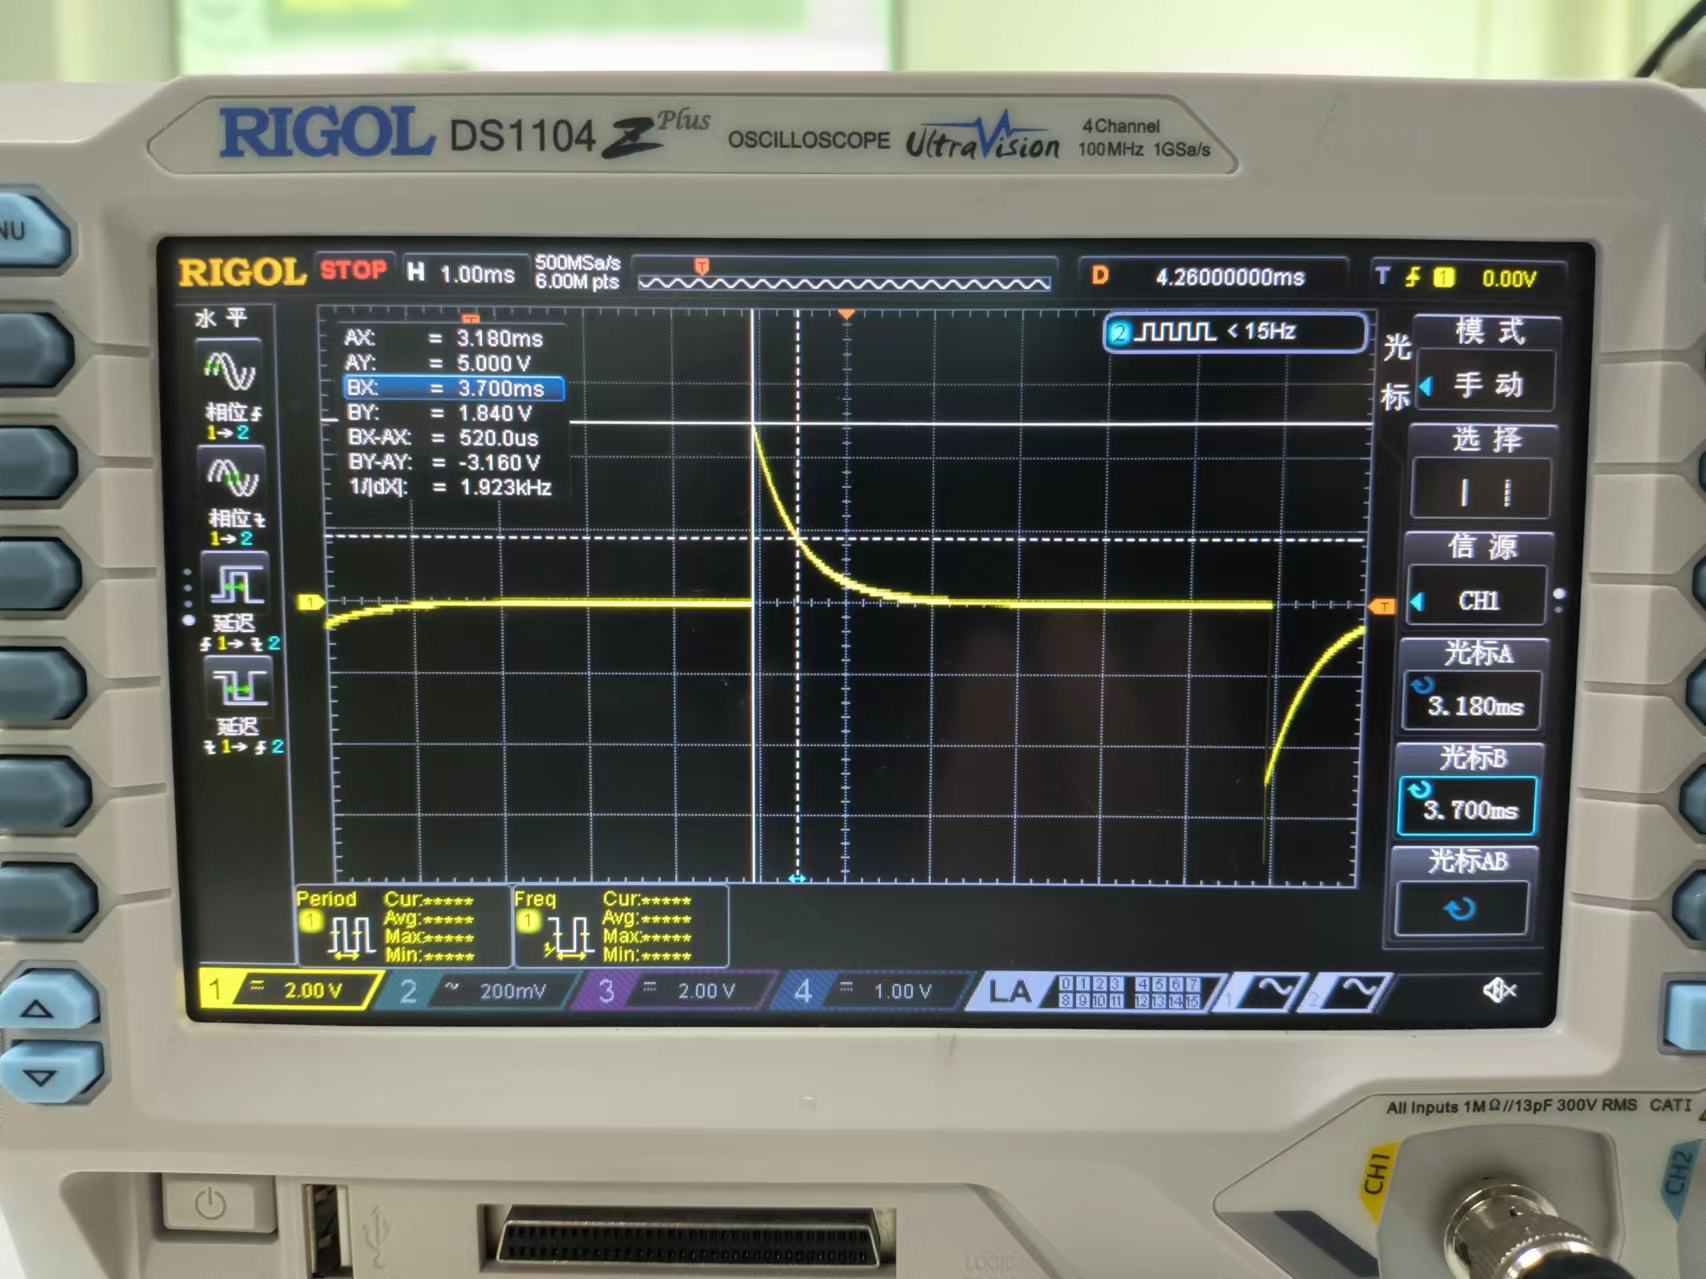
\includegraphics[width=0.35\textwidth]{graph2-12.jpg}\label{fig:graph3-1-1b}}
			\quad
			\caption{RC微分电路波形图}
			\label{fig:graph3-1-1}
		\end{figure}
		
		
		这两张图片(\cref{fig:graph3-1-1a}、\cref{fig:graph3-1-1b})显示的是示波器屏幕,上面展示了输入方波信号到RC(电阻-电容)微分电路后的输出波形。示波器测量的是RC电路输出波形随时间变化的电压。


		
		在RC电路中,当输入方波信号时,电容器将通过电阻充电和放电。RC时间常数$\tau$决定了电容器的充放电速率,时间常数越小,电容器的充放电速度就越快。
		
		我们可以从每张图片中分析如下:
		
		\cref{fig:graph3-1-1a}中:
		\begin{enumerate}
			\item 电阻值为2.4 kΩ(2400 Ω)。
			\item 曲线相当陡峭,表示充电和放电周期较快。
			\item 峰-峰值电压约为5.03 V。
			\item 频率为4.167 kHz,表明信号完成一个周期的频率。
		\end{enumerate}

		\cref{fig:graph3-1-1b}中:
		\begin{enumerate}
			\item 电阻值为5.1 kΩ(5100 Ω)。
			\item 曲线比第一张图片(\cref{fig:graph3-1-1a})中的曲线不那么陡峭,表明由于时间常数较大,响应速度较慢。
			\item 峰-峰值电压仍然在5V左右。
			\item 频率为1.923 kHz,与较大的电阻值相符,表明充放电周期较慢。
		\end{enumerate}

		
		对比两者,可以看到电阻较大(5.1 kΩ)时,示波器上的曲线不如电阻较小(2.4 kΩ)时的曲线陡峭。这是因为较高的电阻会减慢电容器的充放电速率,导致微分效应不那么显著,时间常数较大,因此电容器电压变化的斜率更为平缓。
		
		需要注意的关键点是:
		\begin{enumerate}
			\item 输出波形的振幅没有显著变化,因为它主要由输入信号和电容值决定。
			\item 输出信号的频率与输入频率相对应,但由于RC电路的微分作用,波形形状发生了变化。
			\item 电阻值更高时,输出信号的上升沿和下降沿更加渐进,显示出由于电容器上电压变化速率较慢的“圆滑”响应。
			
		\end{enumerate}

		
		\begin{figure}[htbp]
			\centering
			\subfloat[$R=3000\Omega$]
			{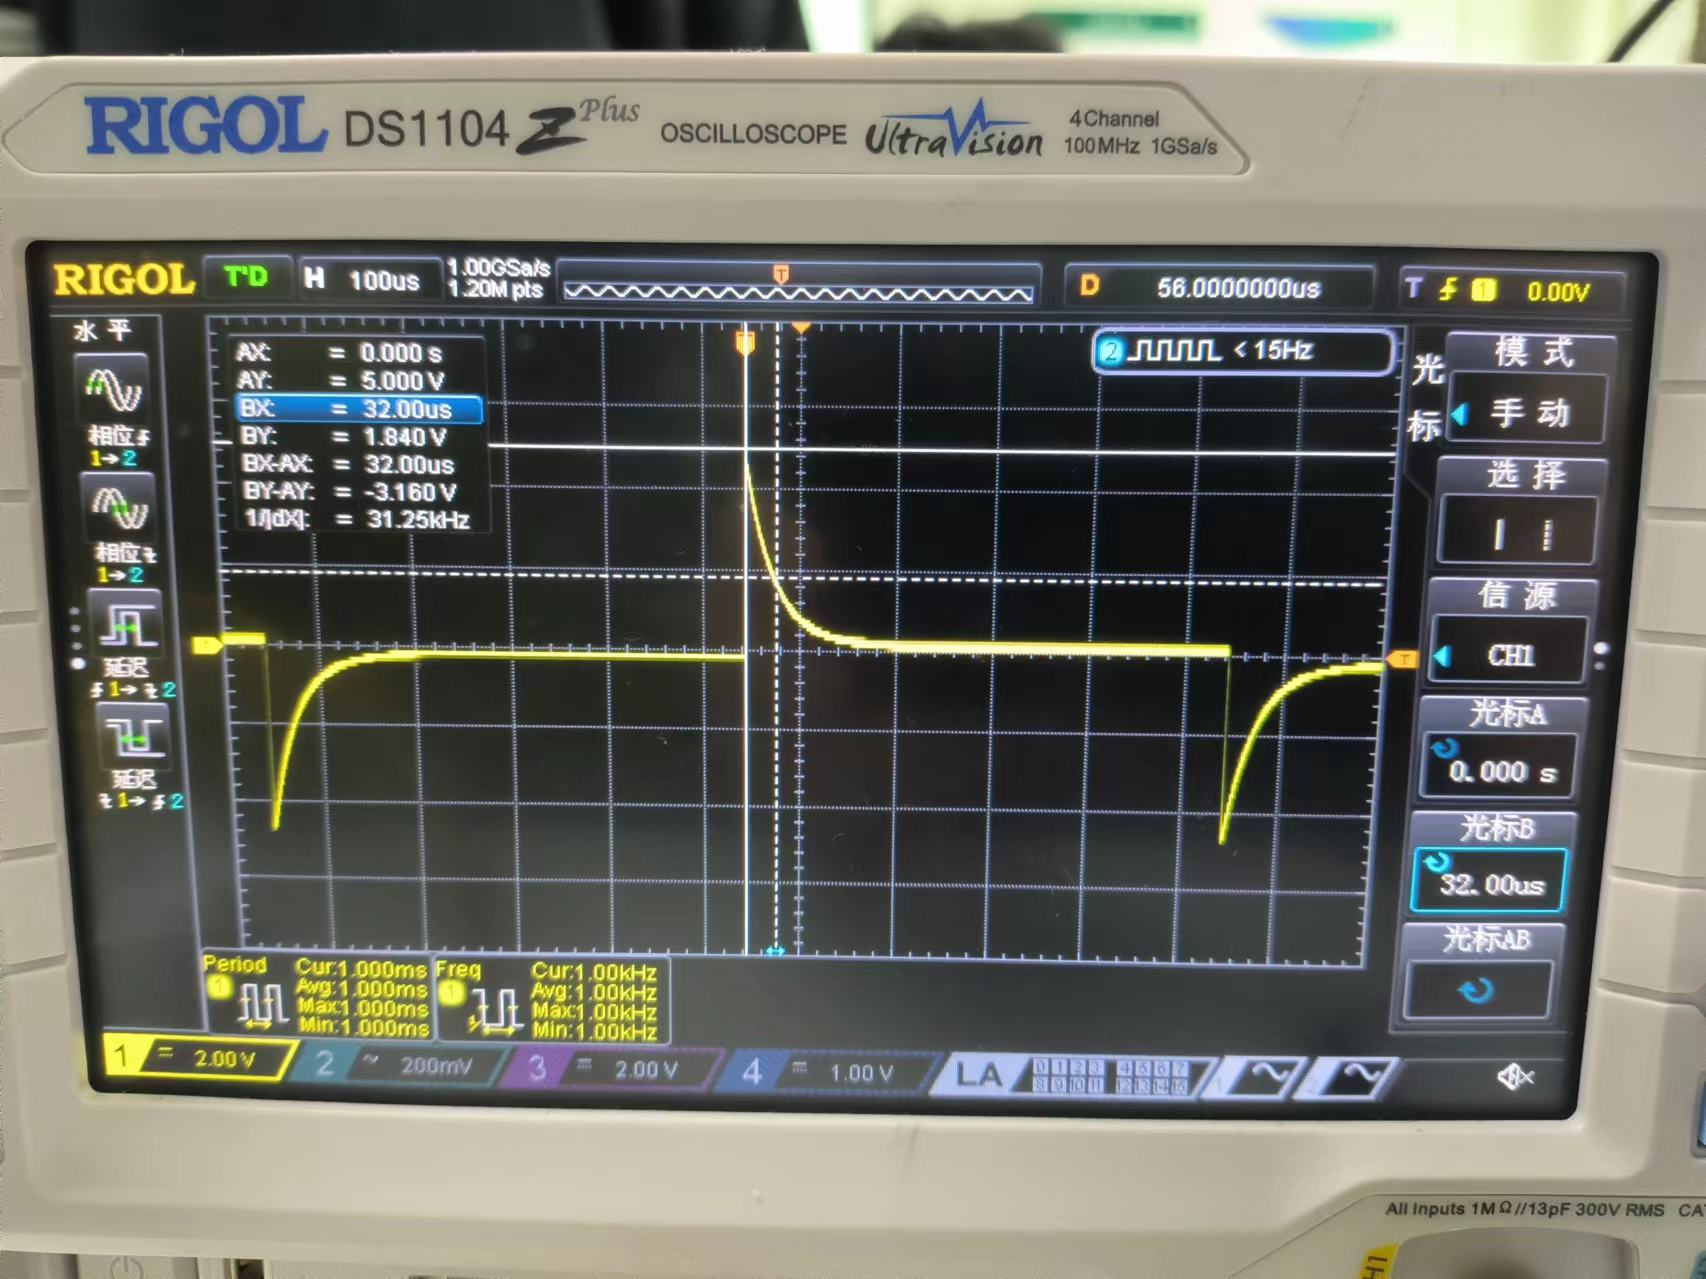
\includegraphics[width=0.35\textwidth]{graph2-21.jpg}\label{fig:graph3-1-2a}}
			\quad
			\subfloat[$R=5000\Omega$]
			{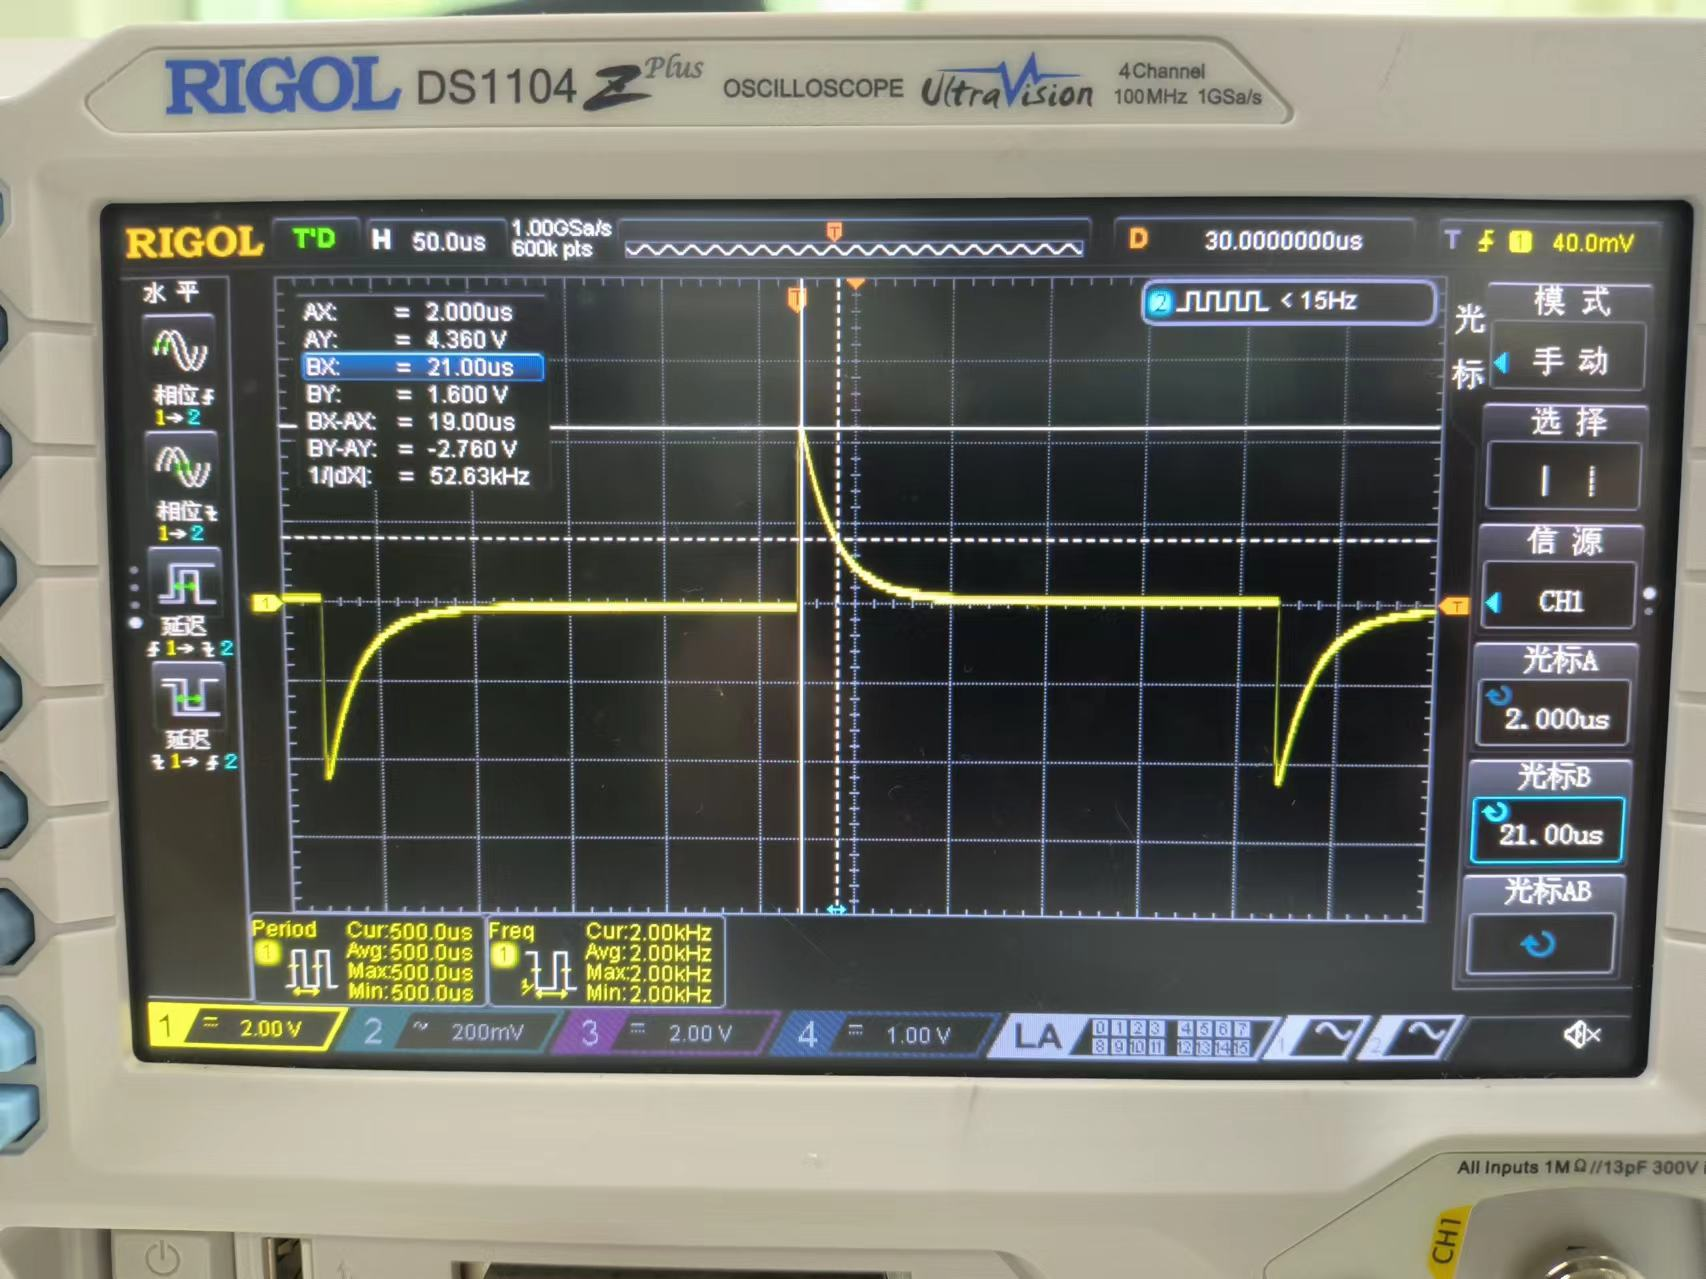
\includegraphics[width=0.35\textwidth]{graph2-22.jpg}\label{fig:graph3-1-2b}}
			\quad
			\caption{RL微分电路波形图}
			\label{fig:graph3-1-2}
		\end{figure}
		
		这两张图片(\cref{fig:graph3-1-2a}、\cref{fig:graph3-1-2b})显示的是示波器屏幕,上面展示了输入方波信号到RL(电阻-电感)微分电路后的输出波形。这类电路中的电感器L在电流变化时会产生阻抗,而这种阻抗与电流变化的速率有关。
		
		在RL电路中,电感L会根据输入信号的变化来抵抗电流的改变。当电流突然增加时,电感会产生一个抵抗变化的电压,这就是为什么当方波信号上升时,我们会在示波器上看到一个尖峰。电阻R决定了电路中电流变化的速率。
		
		\cref{fig:graph3-1-2a}中:
		\begin{enumerate}
			\item 电阻值为3 kΩ(3000 Ω)。
			\item 在方波上升沿和下降沿处,输出信号显示了明显的尖峰。
			\item 这些尖峰表明电感器在电流快速变化时产生了较高的抗变化电压。
			\item 输出信号的峰值约为5 V,频率为31.25 kHz。
		\end{enumerate}
	
		
		\cref{fig:graph3-1-2b}中:
		\begin{enumerate}
			\item 电阻值为5 kΩ(5000 Ω)。
			\item 尖峰的幅度相对第一张图片来说有所减小,表明电感器产生的抗变化电压较低。
			\item 这是因为电阻增加,使得电流变化的速率减慢,因此电感器抵抗变化的反应也减弱了。
			\item 输出信号的峰值约为4.36 V,频率为52.63 kHz。
		\end{enumerate}

		
		比较两个输出信号:
		\begin{enumerate}
			\item 在电阻较小的情况下(3 kΩ),电感器对电流变化的反应更为迅速和强烈,导致尖峰更加明显。
			\item 当电阻增加到5 kΩ时,电感器产生的抗变化电压降低,尖峰的幅度也随之减小。
		\end{enumerate}

	
		
		\item 积分电路波形比对
		
		\begin{figure}[htbp]
			\centering
			\subfloat[$T=500\mu s$]
			{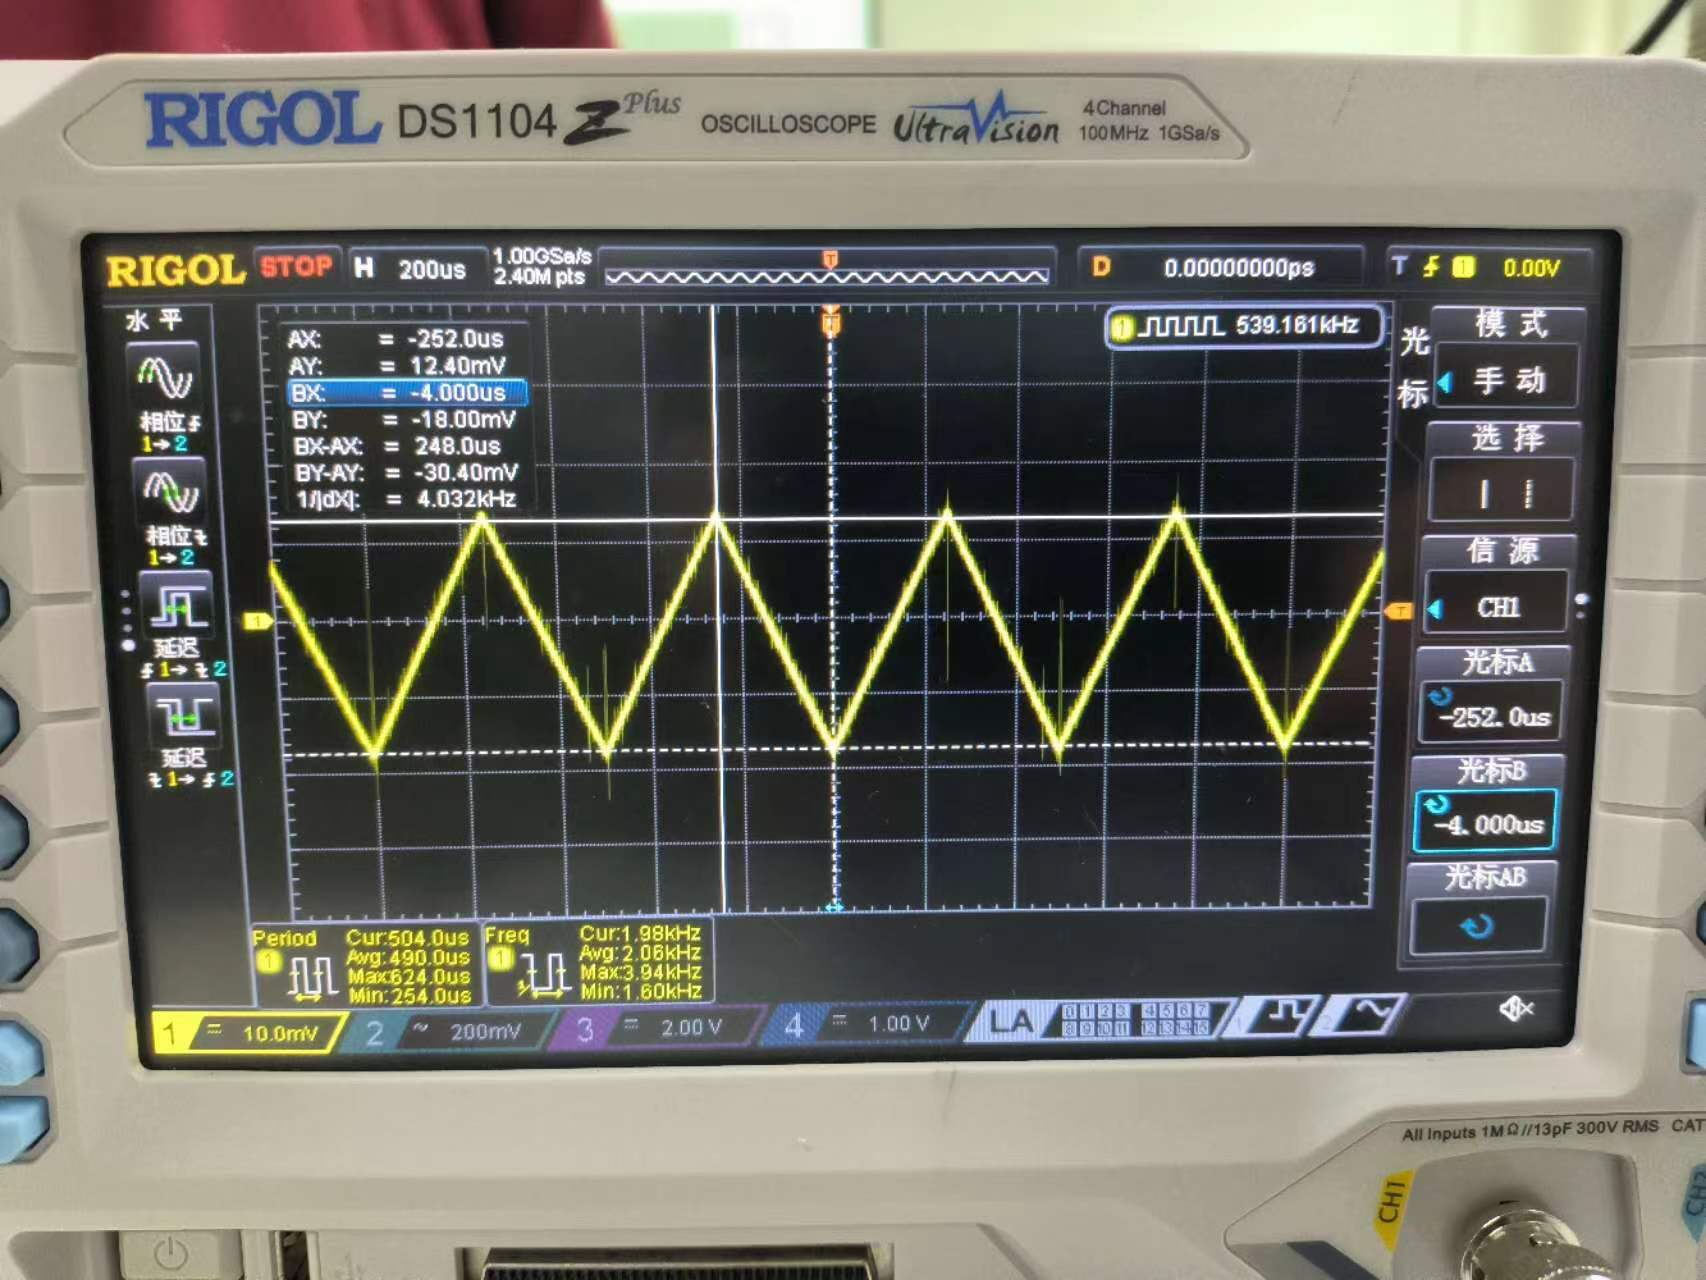
\includegraphics[width=0.3\textwidth]{graph3-2-1.jpg}\label{fig:graph3-2a}}
			\quad
			\subfloat[$T=970\mu s$]
			{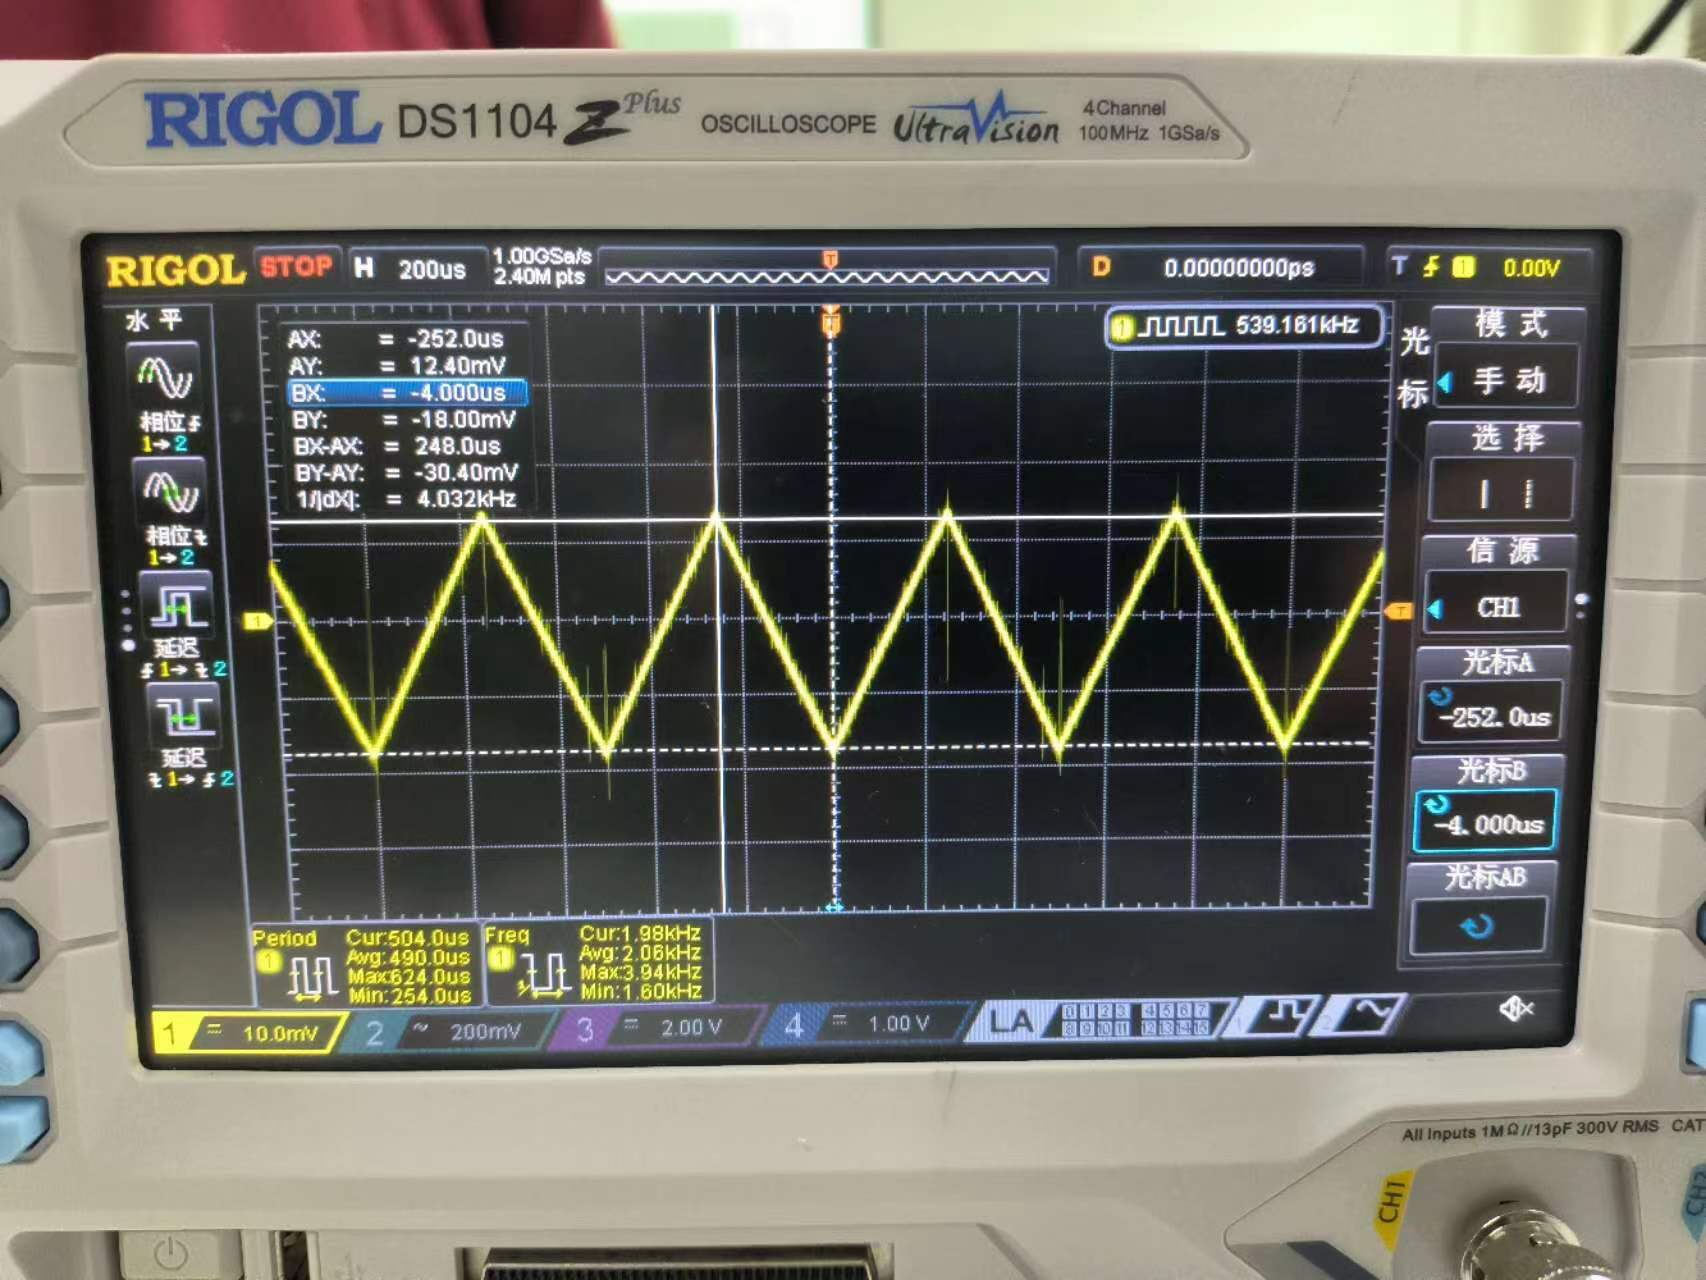
\includegraphics[width=0.3\textwidth]{graph3-2-2.jpg}\label{fig:graph3-2b}}
			\quad
			\subfloat[$T=25\mu s$]
			{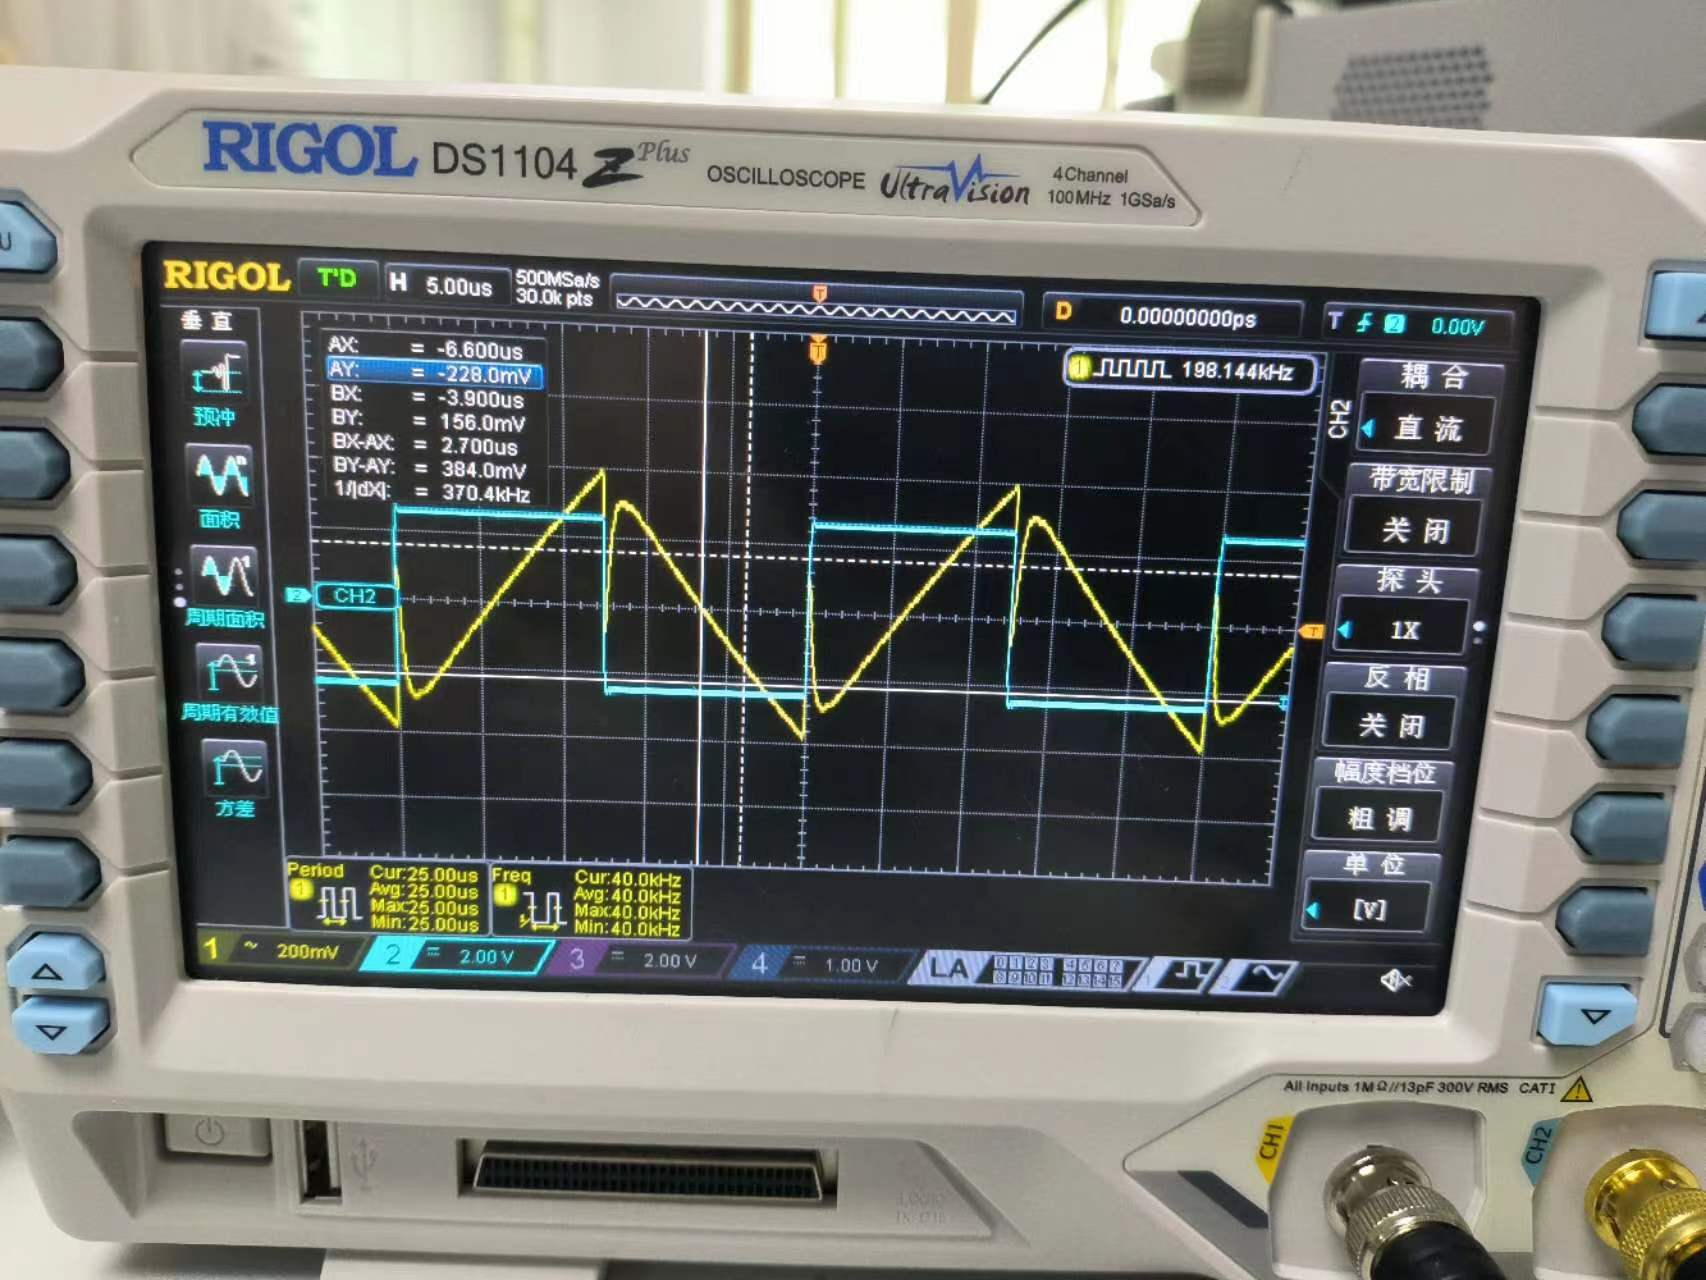
\includegraphics[width=0.3\textwidth]{graph3-2-3.jpg}\label{fig:graph3-2c}}
			\quad
			\caption{三角波波形}
			\label{fig:graph3-2}
		\end{figure}


		从这三张图片来看,我们可以观察到输入方波信号到积分电路后的输出信号。积分电路通常由电阻和电容组成,能够将输入信号的变化率积分,从而在输出端产生相应的波形。
		
		在积分电路中,方波输入会导致电容器逐渐充电和放电,产生一个三角波形的输出。理想情况下,方波的每个上升沿和下降沿将在输出中对应为三角波的上升和下降斜坡。
		
		对比分析这两个输出信号:

		\cref{fig:graph3-2a}中:
		\begin{enumerate}
			\item 输出信号为三角波形,反映了方波信号的积分特性。
			\item 可以看出波形的周期大概是500微秒左右,频率约为2 kHz。
		\end{enumerate}

		% - 三角波的峰值电压大约为12.4 V,表明在积分过程中电压变化的幅度。
		
		\cref{fig:graph3-2b}中:
		\begin{enumerate}
			\item 这张图片同样显示了方波的积分波形,是一个清晰的三角波。
			\item 波形的周期大概是970微秒,频率约为1 kHz。
		\end{enumerate}

		% - 三角波的峰值电压大约为13.20 V,这可能是由于输入信号电压的不同或电路参数的差异所致。
		
		比较两者:
		\begin{enumerate}
			\item 两个波形都保持了三角波的特征,这与积分电路的工作原理相符合。
			\item 第一张图片中的三角波比第二张图片的频率高,表明输入信号的频率更高或者积分时间常数更小。
			\item 第二张图片中的三角波频率较低,可能是因为使用了不同的电路参数,如更大的电容或者更小的电阻,导致积分时间常数增大。
		\end{enumerate}

		
		通常情况下,积分时间常数(由电路中的电阻R和电容C决定)会影响三角波的斜率和宽度。电阻或电容的增加都会增大积分时间常数,导致波形展宽。由于没有提供电路的确切参数,只能根据示波器上显示的波形进行推测。
		
		\cref{fig:graph3-2c}中:
		\begin{enumerate}
			\item 在第三张图片中,我们看到一个不同的波形,它显示了积分效应但波形出现了畸变,可能是由于电路参数或示波器设置的不同造成的。
			\item 这张图片中的周期和频率与前两张图片有显著不同,显示了更低的频率(大约为370 kHz)和不同的波形特征。
		\end{enumerate}

		% - 波形的峰值电压大约为2.38 V,比前两张图片的峰值电压低,这可能是由于输入信号强度不同或者电路中的电阻电容值有所变化。
		
		比较所有三张图片,我们可以看到输入方波的积分效应在波形上的体现,虽然具体的波形特征可能因电路参数和输入信号的不同而有所变化。
		
		\item 微分电路与积分电路的波形比对
		

		\begin{figure}[htbp]
			\centering
			\subfloat[微分电路]
			{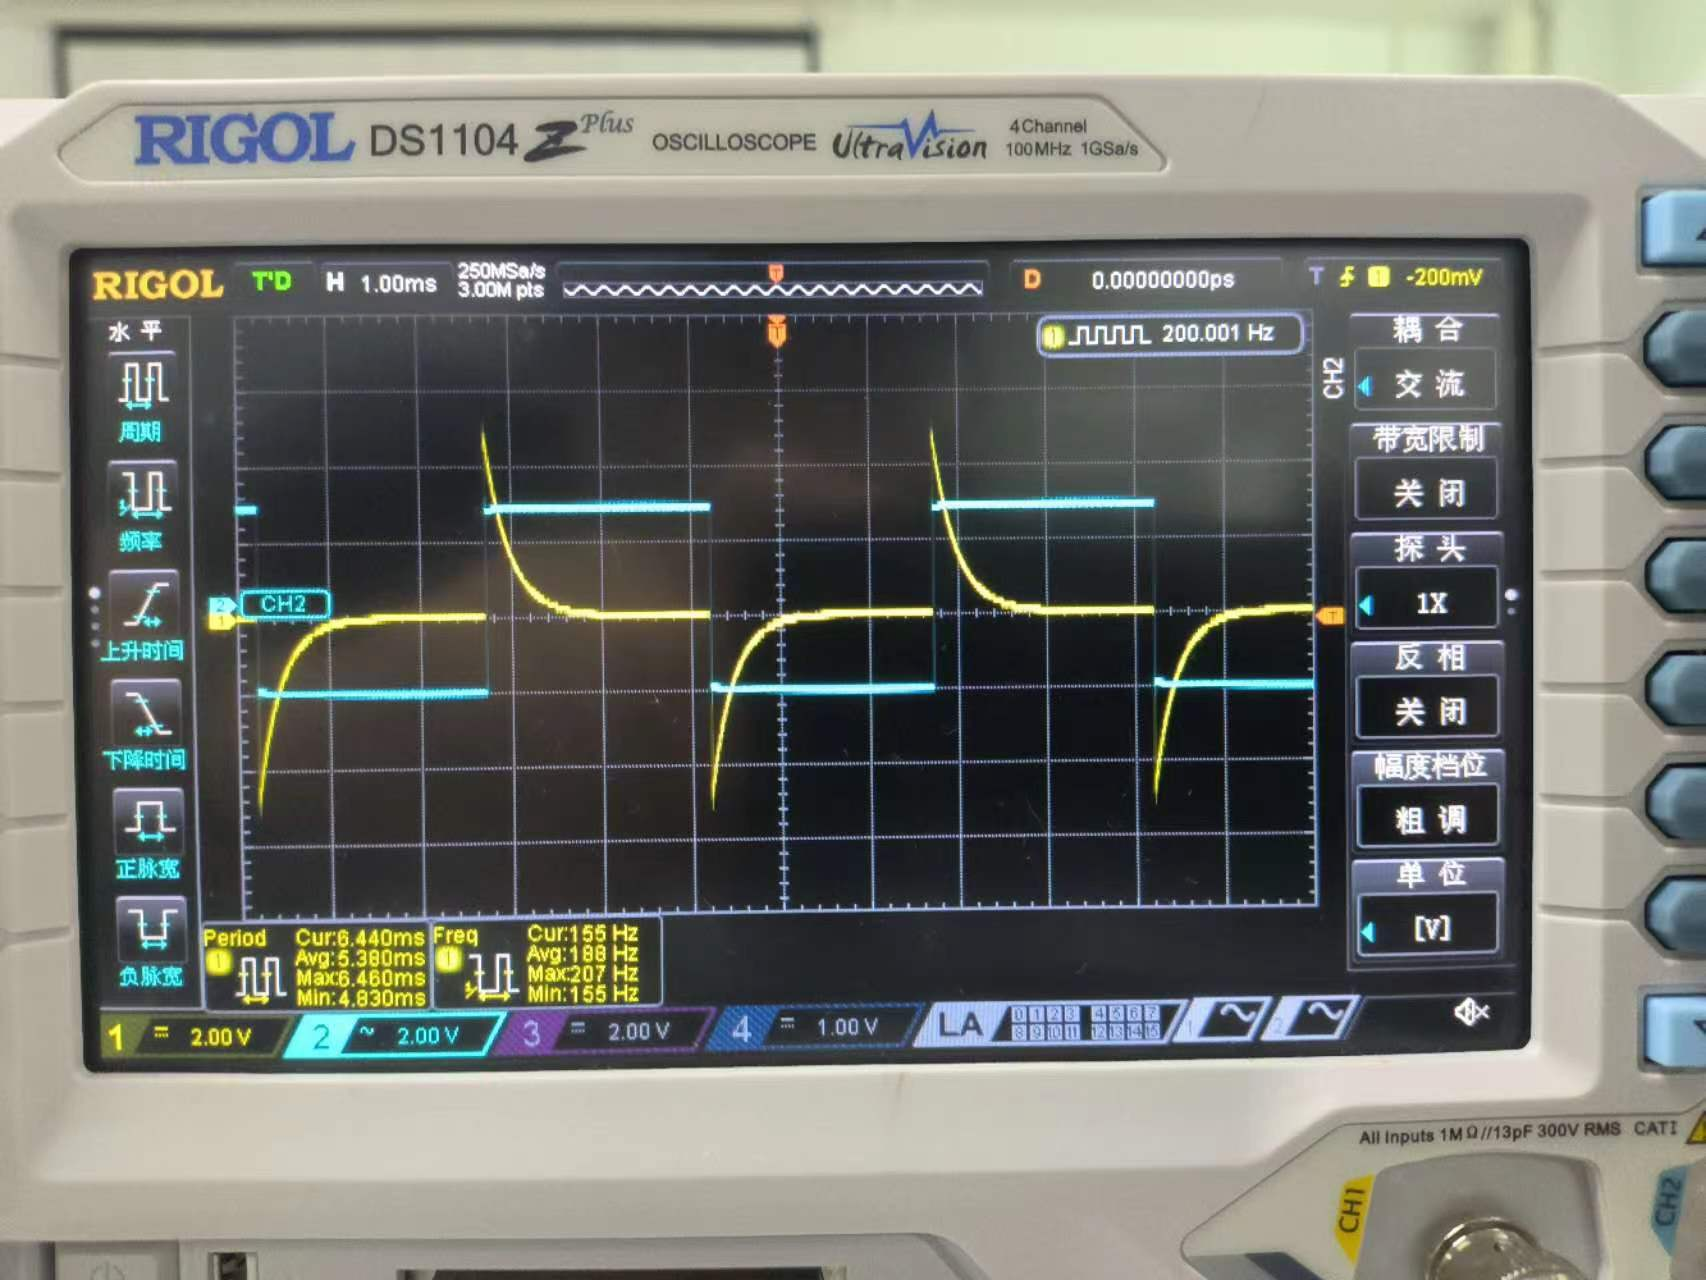
\includegraphics[width=0.35\textwidth]{graph3-3-2.jpg}\label{fig:graph3-3-1}}
			\quad
			\subfloat[积分电路]
			{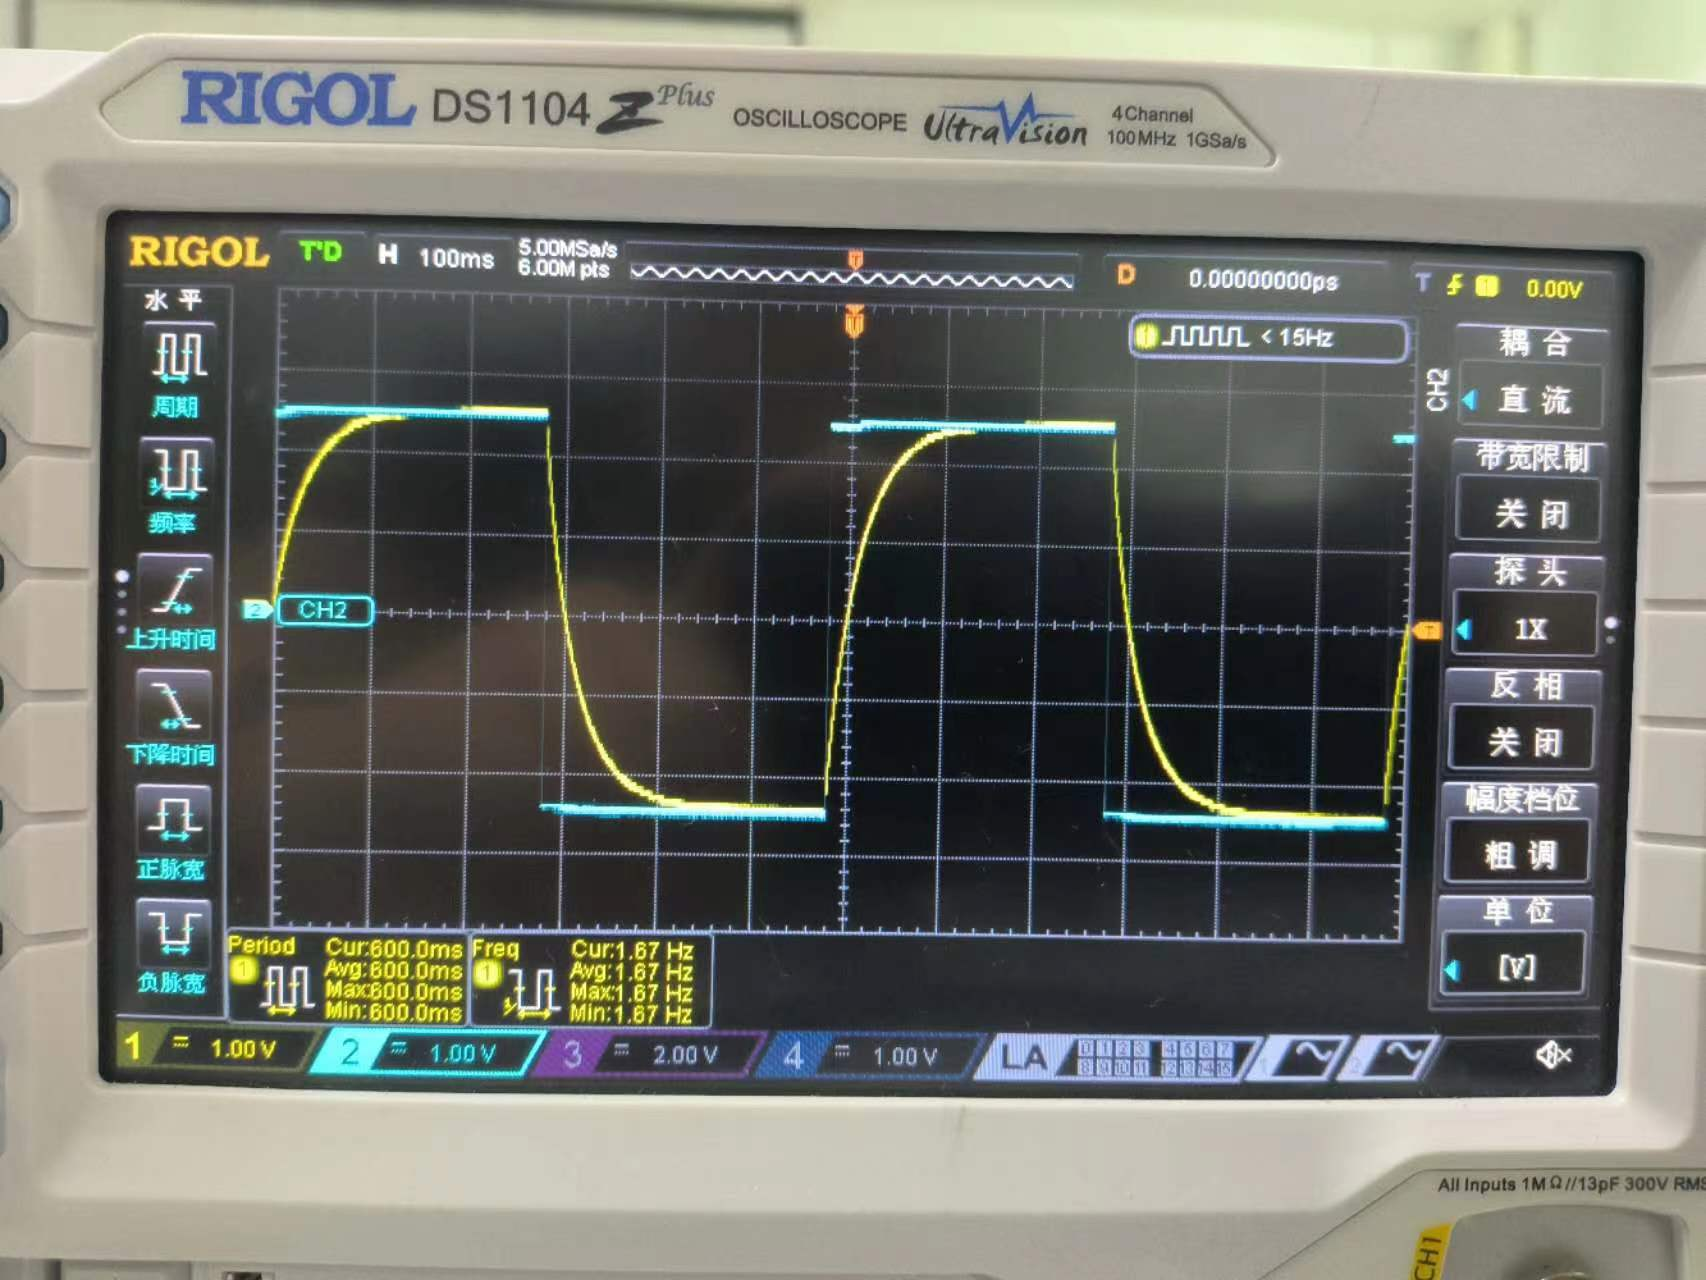
\includegraphics[width=0.35\textwidth]{graph3-3-1.jpg}\label{fig:graph3-3-2}}
			\quad
			\caption{微分电路与积分电路的波形比对}
			\label{fig:graph3-3}
		\end{figure}
		
		从提供的两张示波器屏幕截图中,我们可以比较微分电路和积分电路在输入方波信号后的响应波形。
		
		\cref{fig:graph3-3-1}中:
		\begin{enumerate}
			\item 微分电路的输出波形在每个方波的边缘处产生尖峰,这是因为微分电路对信号变化率的响应。
			\item 当方波从低到高跳变时,电路输出一个正向的尖峰;当方波从高到低跳变时,电路输出一个负向的尖峰。
			\item 这种波形表示微分电路在信号变化时生成一个短暂的高电压。
		\end{enumerate}

		
		\cref{fig:graph3-3-2}中:
		\begin{enumerate}
			\item 积分电路的输出波形为三角波,这是因为积分电路对输入信号进行时间积分。
			\item 方波的每个上升沿和下降沿导致三角波的斜率相应地上升或下降。
			\item 三角波的顶点对应于方波的高点和低点,其幅度和方波的时间宽度相关。
		\end{enumerate}

		
		比对分析:
		\begin{enumerate}
			\item 微分电路响应快速信号变化,而积分电路则对信号持续时间进行积分。
			\item 微分电路产生的是尖锐的脉冲波形,对应于输入信号的快速变化;积分电路产生的是平滑的三角波形,其斜率对应于输入信号的持续时间。
			\item 从波形的外观来看,微分电路产生的尖峰在视觉上更加突出,而积分电路产生的三角波则显示了输入信号的整体形状。
		\end{enumerate}

		
		这两种电路在信号处理中扮演了不同的角色:微分电路常用于强调信号的变化,比如在边缘检测中;而积分电路则用于平滑信号或者计算信号的累积,如在模拟积分器中。
	\end{enumerate}
	
	%
	\subsubsection{时间常数测量的误差分析}
	\begin{enumerate}
		\item 比较测量值与理论值,计算相对误差如\cref{tab:tab2}所示。
		
		\begin{table}[h]
			\centering
			\caption{电路时间常数误差分析}
			\label{tab:tab2}
			\begin{tabular}{|c|c|c|c|c|}
				\hline
				电路 & 时间常数测量值 & 时间常数理论值 & 单位 & 相对误差 \\
				\hline
				RC微分 2.4kΩ & 240.00 & 240 & $\mu s$ & 0.00\% \\
				RC微分 5.1kΩ & 0.52 & 0.51 & ms & 1.96\% \\
				RL微分 3kΩ & 32.00 & 30 & $\mu s$ & 6.67\% \\
				RL微分 5.1kΩ & 19.00 & 20 & $\mu s$ & -5.00\% \\
				RL积分 2.4kΩ & 37.00 & 41 & $\mu s$ & -9.76\% \\
				RL积分 5.1kΩ & 16.80 & 20 & $\mu s$ & -16.00\% \\
				RC积分 3kΩ & 28.00 & 30 & ms & -6.67\% \\
				RC积分 5.1kΩ & 49.00 & 51 & ms & -3.92\% \\
				\hline
			\end{tabular}
		\end{table}
		
		\item 首先,让我们审视这些数据并评估相对误差情况:
		
		\begin{enumerate}
			\item 对于RC微分电路:2.4kΩ电阻的时间常数测量值与理论值完全匹配,相对误差为0.00\%;5.1kΩ电阻的时间常数测量值的相对误差为1.96\%,略高于理想情况。
			
			\item 对于RL微分电路:3kΩ电阻的时间常数测量值的相对误差为6.67\%,略高于理想情况;5.1kΩ电阻的时间常数测量值的相对误差为-5.00\%,显示出一定的低估。
			
			\item 对于RL积分电路:2.4kΩ电阻的时间常数测量值的相对误差为-9.76\%,显示出明显的低估;5.1kΩ电阻的时间常数测量值的相对误差为-16.00\%,也显示出明显的低估。
			
			\item 对于RC积分电路:3kΩ电阻的时间常数测量值的相对误差为-6.67\%,显示出一定的低估;5.1kΩ电阻的时间常数测量值的相对误差为-3.92\%,显示出一定的低估。
		\end{enumerate}
		
		\item 可能的误差来源:
		
		\begin{enumerate}
			\item \textbf{测量仪器的误差}:测量设备可能存在固有的误差,例如示波器的分辨率限制、数字测量设备的精度等。这种误差会在实验数据中引入一定的偏差。
			
			\item \textbf{元件参数的测量误差}:电阻、电容、电感等元件的实际值可能与标称值略有不同。特别是在电路设计中使用的元件值与实际测量到的值之间可能存在差异。
			
			\item \textbf{电路搭建的误差}:电路的搭建过程可能引入连接不良、松动、焊接不良等问题,导致电路性能不稳定或与理论预期不符。
			
			\item \textbf{环境条件的影响}:环境条件如温度、湿度等因素可能对电路的性能产生影响,尤其是对某些元件(如电容)的影响可能较大。
			
			\item \textbf{测量方法的不确定性}:测量时间常数的方法可能影响测量结果,不同的测量方法可能会引入不同程度的误差。
		\end{enumerate}
	\end{enumerate}
	
	%
	\subsubsection{关于微分、积分电路的进一步讨论}
	\begin{enumerate}
		\item 理论分析
		
		以RC积分电路为例,当采样时间远远小于时间常数$T_p<<\tau$时,由近似可得$V(t)=V_0e^{-\frac{t}{\tau}}=V_0(1-\frac{t}{\tau})$,这说明它将方波变为了三角波,斜率正好是$-\frac{V_0}{\tau}$。
		
		\item 电路仿真
		
		根据上述理论分析,我们利用仿真软件multisim作了进一步探究,如\cref{fig:figA1}和\cref{fig:figA3}所示。
		
		\begin{figure}[htbp]
			\centering
			\subfloat[]{
				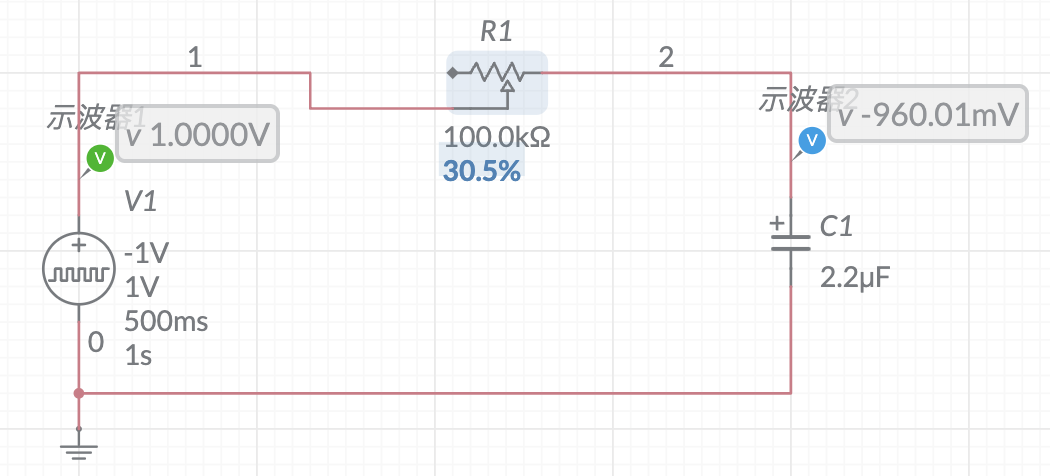
\includegraphics[width=0.4\textwidth]{ET1_5GraA1.png}
			}
			\subfloat[]{
				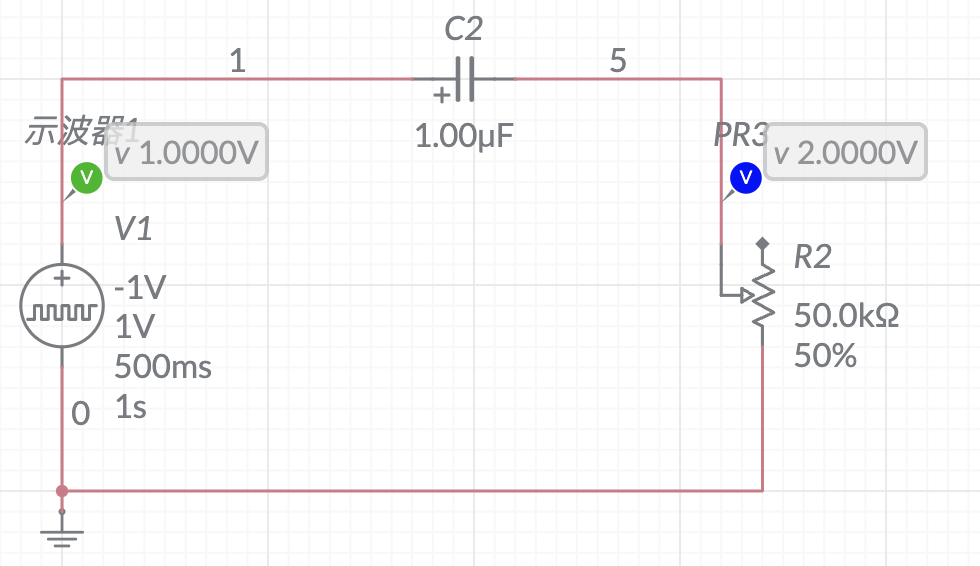
\includegraphics[width=0.4\textwidth]{ET1_5GraA2.png}
			}
			\caption{仿真电路}
			\label{fig:figA1}			
		\end{figure}
		
		\begin{figure}[htbp]
			\centering
			\subfloat[]{
				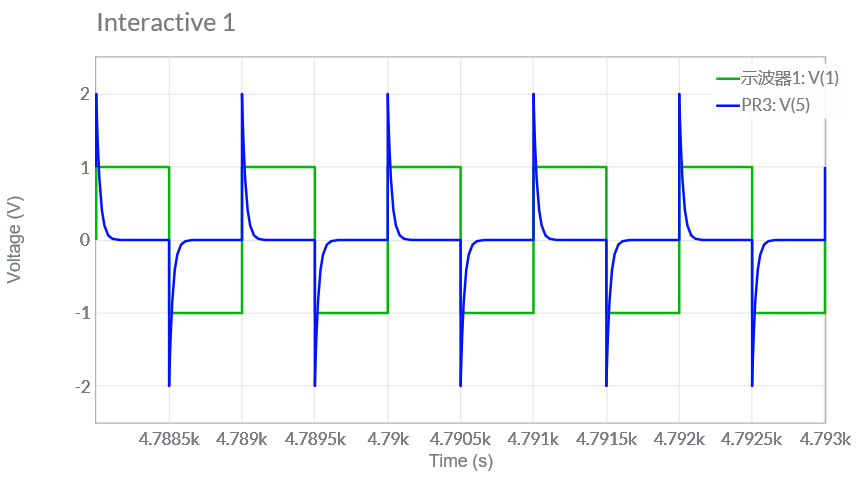
\includegraphics[width=0.4\textwidth]{ET1_5GraA3.png}
			}
			\subfloat[]{
				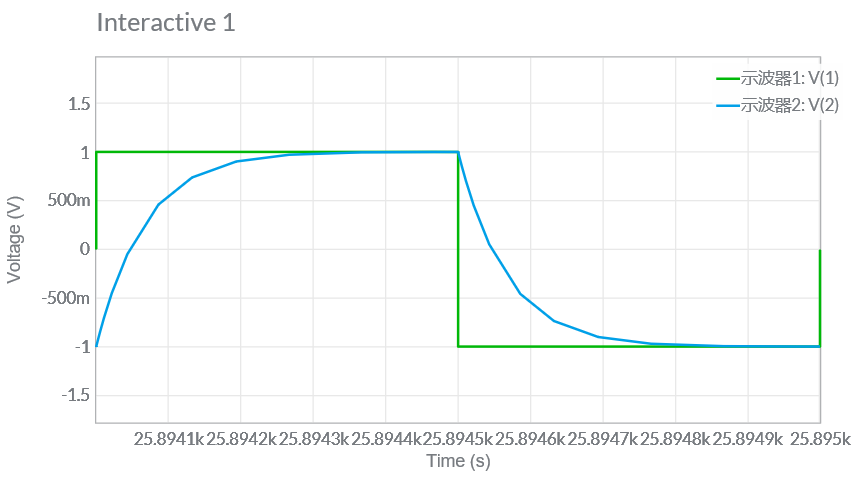
\includegraphics[width=0.4\textwidth]{ET1_5GraA4.png}
			}
			\caption{仿真输出波形}
			\label{fig:figA3}			
		\end{figure}
		
		\item 拓展研究
		
		根据上述理论分析,我们也对实际测量的RC积分电路三角波作了分析,如\cref{tab:tab3}所示。可以看出,这样的理论近似还不够好。
		
		\begin{table}[h]
			\centering
			\caption{时间常数测量结果及相对误差}
			\label{tab:tab3}
			\begin{tabular}{|c|c|c|}
				\hline
				时间常数理论值/微秒 & 采样时间/微秒 & 方波电压/V\\
				\hline
				30.00 & 500.00 & 5.00\\
				\hline
				BX-AX/微秒 & BY-AY/mV & 斜率的倒数\\
				\hline
				248.00 & -30.40 & -8.16\\
				\hline
				时间常数测量值 & 相对误差 & \\
				\hline
				40.79 & 35.96\% & \\
				\hline
			\end{tabular}
		\end{table}
		
		
	\end{enumerate}
		
	% ---
	
	% 实验后思考题
	%\subsection{实验后思考题}
	
	% ---
	
	
	% 结语部分
	\clearpage
	
	% 小标题
	\section{ET1-5 一阶电路暂态过程的研究 \quad\heiti 结语}
	% ---
	
	% 总结、杂谈与致谢
	\subsection{实验心得和体会、意见建议等}
	\begin{enumerate}
		\item 实验心得体会
			\begin{enumerate}
				\item 理论与实践的结合:通过这次实验,我对电路理论有了更深刻的理解。实际操作中,我能够将抽象的理论知识应用到具体的电路设计中,这让我认识到了学习理论知识的重要性。
				
				\item 技术技能的提高:在实验过程中,我对电路的搭建和测量技术变得更加熟练。在这次实验中,我们大量的使用了信号发生器和示波器,通过这个实验我们基本掌握了这两个仪器的使用方法。
				
			\end{enumerate}
		
		\item 意见和建议
			\begin{enumerate}
				\item 完善实验指导:希望能够对实验指导书进行更新,使其内容更加详尽,尤其是在描述实验步骤时。同时,对于可能遇到的问题,提供更多的提示和解决策略。
				
				\item 设备的定期维护:建议学校定期对实验室设备进行维护和升级,以避免实验中出现设备故障,影响实验进度和结果。
				

			\end{enumerate}
			
		\item 感谢老师能阅读这篇还有很多不足的实验报告,希望老师能指出做得不好的地方;祝老师身体健康、生活幸福、工作顺利!
	\end{enumerate}
	% ---
	
	% 参考文献
	\subsection{参考文献}
	[1] 维基百科 https://zh.wikipedia.org
	
	[2] 沈韩.基础物理实验.——北京:科学出版社,2015.2 ISBN:978-7-03-043311-4
	
	% ---
	
	% 附件
	\subsection{附件及实验相关的软硬件资料等}
	试验台桌面整理如\cref{fig:table}所示。

		\begin{figure}[htbp]
			\centering
			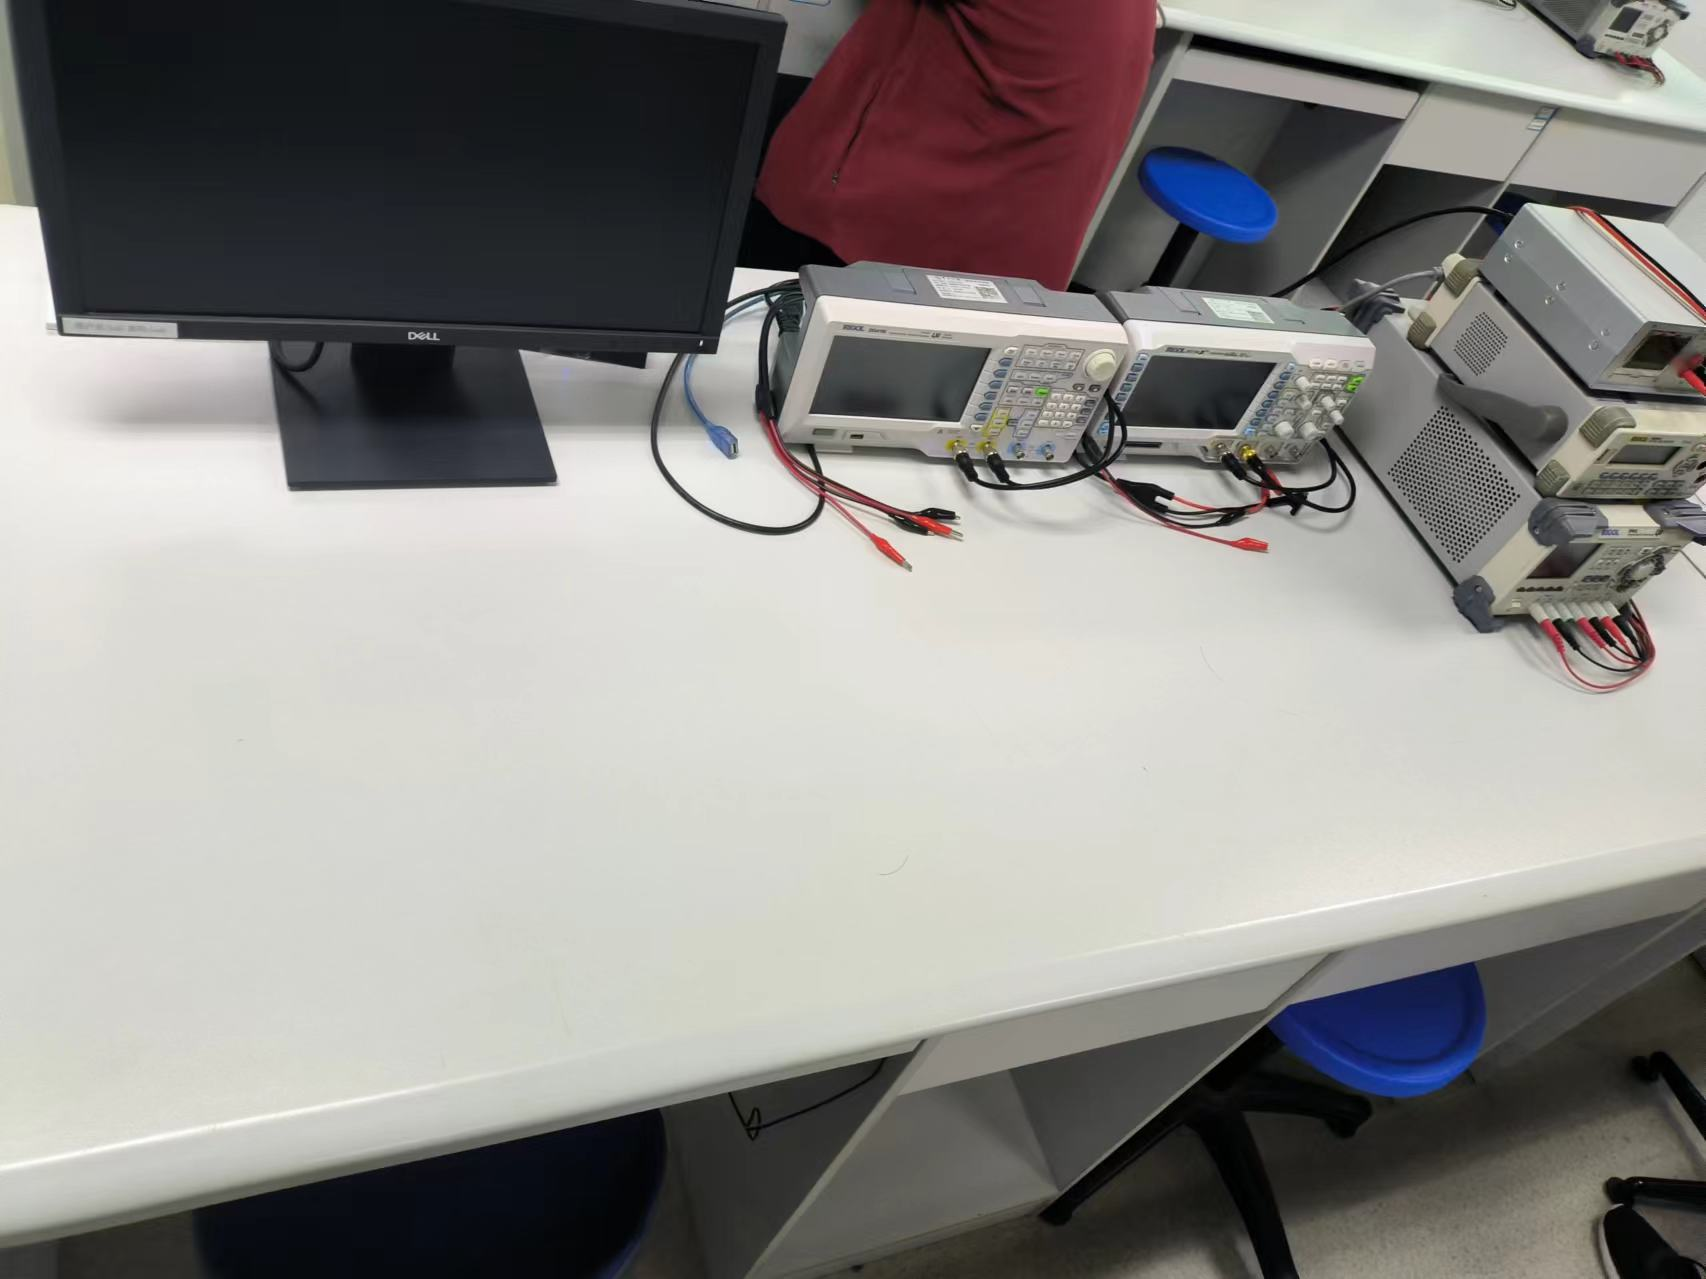
\includegraphics[width=0.5\textwidth]{table.jpg}
			\caption{试验台桌面整理}
			\label{fig:table}
		\end{figure}
	
	实验报告个人签名如\cref{fig:name}。
	
	\begin{figure}[htbp]
		\centering
		\subfloat[]{
			
\includegraphics[width=0.45\textwidth]{name.png}
		}
		\subfloat[]{
			
\includegraphics[width=0.45\textwidth]{name-TaLEs.jpg}
		}
		\caption{个人签名}
		\label{fig:name}			
	\end{figure}
	
	% ---
	
	相关代码已上传至Github。
	
	
	
\end{document}